\chapter{The improved BIPMIN tool}
\label{ch5}

The development of the framework described in the previous chapter aimed at addressing the issues that had emerged with the empirical study with BIPMIN, leading to the development of a new tool and the execution of a second experiment with a similar design, to observe whether a new set of mechanics and a revised evaluation approach could make a gamified tool more effective. The framework was designed with the goal of supporting longitudinal use, implying the need of a specific evaluation procedure aimed at testing its potential benefits over a period of time beyond that of a single experiment. For this purpose, it was decided to redevelop the BIPMIN application, which had already proved the benefits of gamification applied to BPMN modeling, in accordance with the new selection of game mechanics, and to use this new version for the practical activities of the Information System course, where the original tool was tested.

The goal of this new study was to explore a different research direction: instead of comparing the gamified approach with regular modeling activities, the purpose was to observe whether continuous use of a gamified environment would lead to measurable improvements in the students' BPMN modeling knowledge and final performance. This chapter describes how the BIPMIN tool was redesigned according to the new framework and then presents the results of the study, focused on both the overall student perception of the gamified experience and on the empirical evaluation of how the tool impacted the students' grades and learning progression over time. The work described in this chapter has been split into two research articles: a first experience report focused on student perception and lessons learned was presented in \cite{garaccione2024ease}, while the empirical evaluation was described in \cite{garaccione2024esem}.

\section{Limitations of the existing version}

The original empirical study conducted in January 2023 identified a clear set of lessons and issues with the first implementation of the BIPMIN tool that guided the latter part of the PhD course's first year, leading to the implementation of UMLegend.

The first, and most significant, limitation was found in the rigid evaluation engine: despite the introduction of a semantic assessment check for assessing the content of a diagram (element names, types, position in relation to other elements) beyond regular adherence to syntax rules, the reference solution remained constrained to a single target model with limited variability in the set of accepted alternative ways to represent each process part. Many students who had produced a diagram semantically equivalent to the reference but with variations such as different element names, alternative structural choices or unexpected synonyms in part of the names got penalized by the evaluator not recognizing their work as correct, an assessment that would be found as such by a human observer. This resulted in continuous penalization that was in turn identified as the main source of dissatisfaction, resulting in the neutral perception of the overall experience highlighted by the answers to the GAMEX questionnaire; the key lesson found from this issue was that the game mechanics would not work as expected if they relied on an evaluation that students would perceive as unfair. 

Another limitation was connected to the results related to the impact of gamification over syntactic correctness: the original study showed a positive impact on semantic quality, highlighting that gamification could help students produce more correct models, but no similar effect could be observed regarding syntax quality and, consequently, on the benefits related to learning basic BPMN modeling rules. The reason for this result depends on the study's design: by conducting the experiment at the end of the course, students were already knowledgeable about BPMN syntax, especially because of the syntax enforcing feature present in the editor they were used to (Signavio Academic); this meant that students could be considered as experts on the syntactic point of view, highlighting the need to conduct a similar assessment earlier in the course, when students begin facing BPMN problems and need support and assistance to learn the key concepts, which is what gamification could help with and one of the goals of the PhD research.

Lastly, the implementation of the penalty mechanic, which was selected to introduce a negative motivator and discourage students from continuously submitting unchanged solutions, led to excessive frustration due to unexplained feedback behind the errors and consequent inability to understand why certain modeling choices were considered incorrect. 

Overall, the combination of a limited evaluation engine and excessively strict game mechanics led to the experience being seen in a neutral light, reducing the engaging effect of gamification, and the execution of the study at the end of the course limited the ability to assess its educational impact. 

\section{Tool changes according to the UMLegend framework}

After identifying the limitations with the original BIPMIN implementation, development of a new version started during Spring 2023 according to the gamified framework identified with the creation of UMLegend, making sure that both tools would share a common design logic adapted to the specific modeling domains, with the end goal of merging them in a single, multi-purpose educational environment. The development process led to the complete re-implementation of the evaluation engine as well, to extend the tool's ability to assess a diagram's correctness.

The same design choices made for UMLegend applied to the new version of BIPMIN: a separate client interface for teachers was implemented to support long-term course management, allowing for the creation of student profiles, new exercises, and most importantly reference solutions for each exercise, moving forward from the original implementation where solutions were hard-coded with no easy way to change them. On the student side, a homepage was added to allow for profile and avatar customization, as well as easy access to exercises. The implementation of game mechanics according to the UMLegend structure was guided by the new evaluation engine, which was identified as the first necessary change to improve the tool and make it suitable for long-term use.

\subsection{Evaluation Engine}

The behavior behind the new evaluation engine kept the same logic as the version used for the study: the evaluator would have to simulate the behavior of a teacher who looks at a diagram and identifies elements that represent specific parts of the target process and assesses errors such as wrong ordering of elements, elements belonging to different pools/lanes, and incorrect message exchanging.

The use of \textit{Process Parts} as the logical blocks to base a reference solution on remained as the key idea behind the evaluation engine; however, it became obvious after the study that each process part, and each element inside them, had to be assessed separately, with relationships between elements and parts being assessed at a later step in the evaluation, following identification of matching process parts. As a consequence, the data structure that implements reference solutions was restructured to distinguish between structural elements (pools, lanes, sub-processes), process parts, and forbidden elements.

\textit{Business Entities} were added as structures that were used to identify the pools expected to be included in a diagram. For each of them, a unique name was required, to express the corresponding pool both in feedback mechanics and in relationship to other elements in the solution; a set of synonyms could also be specified for each entity, allowing for more ways to express the same concept and leading to a match if a student's diagram included a pool with a name similar enough to either a synonym or the reference name. Furthermore, the ability to specify whether an entity was external pr not, requiring the use of a collapsed pool to represent it, was added, together with the ability to mark an entity as mandatory or as one that can be omitted without causing an error.

\textit{Actors} were used to represent the possible lanes that could be included in a diagram's pools. A unique reference name would identify each actor, with the list of possible synonyms being used as well, and, for each actor, the identifier of its parent pool An actor is considered represented correctly if there is a lane with a similar name to one of the allowed ones, if the parent business entity has a matching pool, and if the matching pool contains the matching lane; in case a matching pool is not found for a given business entity, all actors are automatically considered not found.

\textit{Sub-process} objects were used to identify the corresponding diagram elements that could group together multiple tasks and events inside a larger pool. Each object of this type could specify the parent element (either a pool or another sub-process) and whether it is a regular or an event-triggered sub-process, in which case it was also possible to state whether it could interrupt the parent element or not.

\textit{Forbidden Entities} were used to identify names that could not be used to represent pools or lanes, marking errors such as using names intended for business entities to represent actors (or vice-versa), including actors and entities that do not interact with the process, or representing the system or parts of it as an actor rather than as the entire diagram.

Lastly, the definition of \textit{Process Parts} was completely redone to allow for a more thorough and less strict evaluation: first of all, each part could be represented by multiple alternative groups of elements, where each element could be defined in different alternative ways to support the variability of correct representation. Each given element in a group would have a unique identifier in the solution and state the possible options such as the set of accepted names, the pool and lane the element would belong to, the list of preceding elements, information about message exchanges and boundary-type relationships (type and identifier of the connected element), a description of the element to be used for feedback, and the set of acceptable element-specific information to represent it (e.g., regular tasks and user tasks, message sending events and message sending tasks, interrupting or non-interrupting events, gateways that split or merge multiple flows). An element in a given process part's group is considered matched with a diagram element that has a name similar enough to one of the allowed ones, an accepted type out of the defined set, and that belongs in the intended pool; a process part is considered matched if there is one group where all elements have a match in the diagram, checking exclusively the three conditions, while other constraints are assessed separately and identify other types of errors. 

The decision to keep element matching to the minimum was not only made to make the evaluation engine less strict, reducing the set of necessary information to be correct for a match to the fundamental information, but also to expand on the feedback mechanic, which was limited to simply highlighting which process parts had been found: implementing separate checks on different error types would make it possible to provide additional feedback explanations, helping students fix the more precise details in their diagrams. 

Another decision made to increase the granularity of the feedback mechanisms and thus enhance the educational capabilities of the improved BIPMIN was to define a third category of analysis performed during semantic assessment with the concept of \textit{Closeness} by marking close elements and close process parts, with the former being reference elements in a non-matched process part for which there is a diagram element with a matching name but at least one other matching condition (belonging to the intended pool or being an accepted type) not satisfied, and the latter being process parts that have a match for at least 50\% of the elements but not all, selecting the group with the highest number of matched elements. This would lead to scenarios where students could draw elements that represent an intended purpose but with an incorrect understanding (e.g., using a user task to represent an activity performed automatically instead of a service task or having activities performed by a different business entity or actor than expected) and know what they should change, or representing most of what composes a certain part of the requirements but missing key sections of the interaction; the use of a description for each element in the reference solution serves this purpose, with feedback related to closeness using these descriptions to report the missing elements.

Following the definition of the new reference solution structure, the evaluation procedure was re-implemented to adapt to the new format, keeping the same logic used in the UMLegend tool: a first syntax check used to identify structural errors and point out violations to standard BPMN rules followed by the semantic assessment to identify correct process parts, errors and close elements.

The syntax evaluation kept the original underlying structure by using the \textit{bpmn-js-bpmnlint} library to identify known errors (unnamed elements, processes with no starting or ending events, incorrect use of incoming and outgoing flows), with the addition of new custom rules focused on ensuring only certain elements could launch sequence flows or violations tied of boundary events such as not managing their outgoing flows or attaching them to incorrect elements; the full set of syntactic criteria is presented in Figure \ref{fig:syn_rules}.

\begin{figure}[ht]
    \centering
    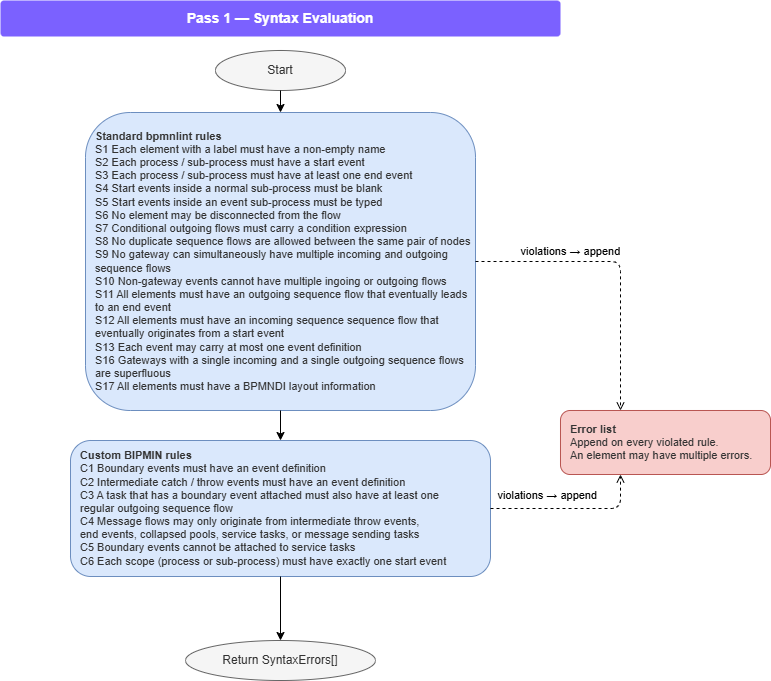
\includegraphics[width=0.75\linewidth]{Template_Latex_ScuDo_Tesi/Chapter5/syn_rules.png}
    \caption{Syntax evaluation rules}
    \label{fig:syn_rules}
\end{figure}

Following a complete syntax assessment, the semantic evaluation takes place by comparing elements in a diagram with the set of reference solutions: the process iterates on the three structural elements (pools, lanes, sub-processes) first and then loops through the process parts; a second iteration on each process part's possible group of elements is performed, looking for the specified elements by continuously filtering the elements in the diagram according to the specified properties. The sorting follows a given order: first, the element type is checked, then name similarity, then by belonging to the expected parent; in case an element has additional constraints that depend on the type such as event definition or gateway type (split or merge), those properties are also added to the filtering procedure. After all groups have been processed and matching parts have been identified, a second evaluation step is performed to identify errors such as elements in the same part being in the wrong order or parts being in the wrong order (identified by the last element of the preceding part not having an outgoing flow to the first element of the following part), and a final step looks at the elements in non-matched parts to look for close elements among diagram elements that do not belong to any part. This process is repeated for each defined reference solution and leads to the computation, together with the list of errors, of a completeness score that depends on the sum of matched entities, actors, sub-processes, and process parts over the total number of such elements; the solution with the highest score is used as the reference and its accompanying feedback is shown to the student. Figure \ref{fig:sem_alg_5} summarizes the semantic evaluation process.

\begin{figure}[ht]
    \centering
    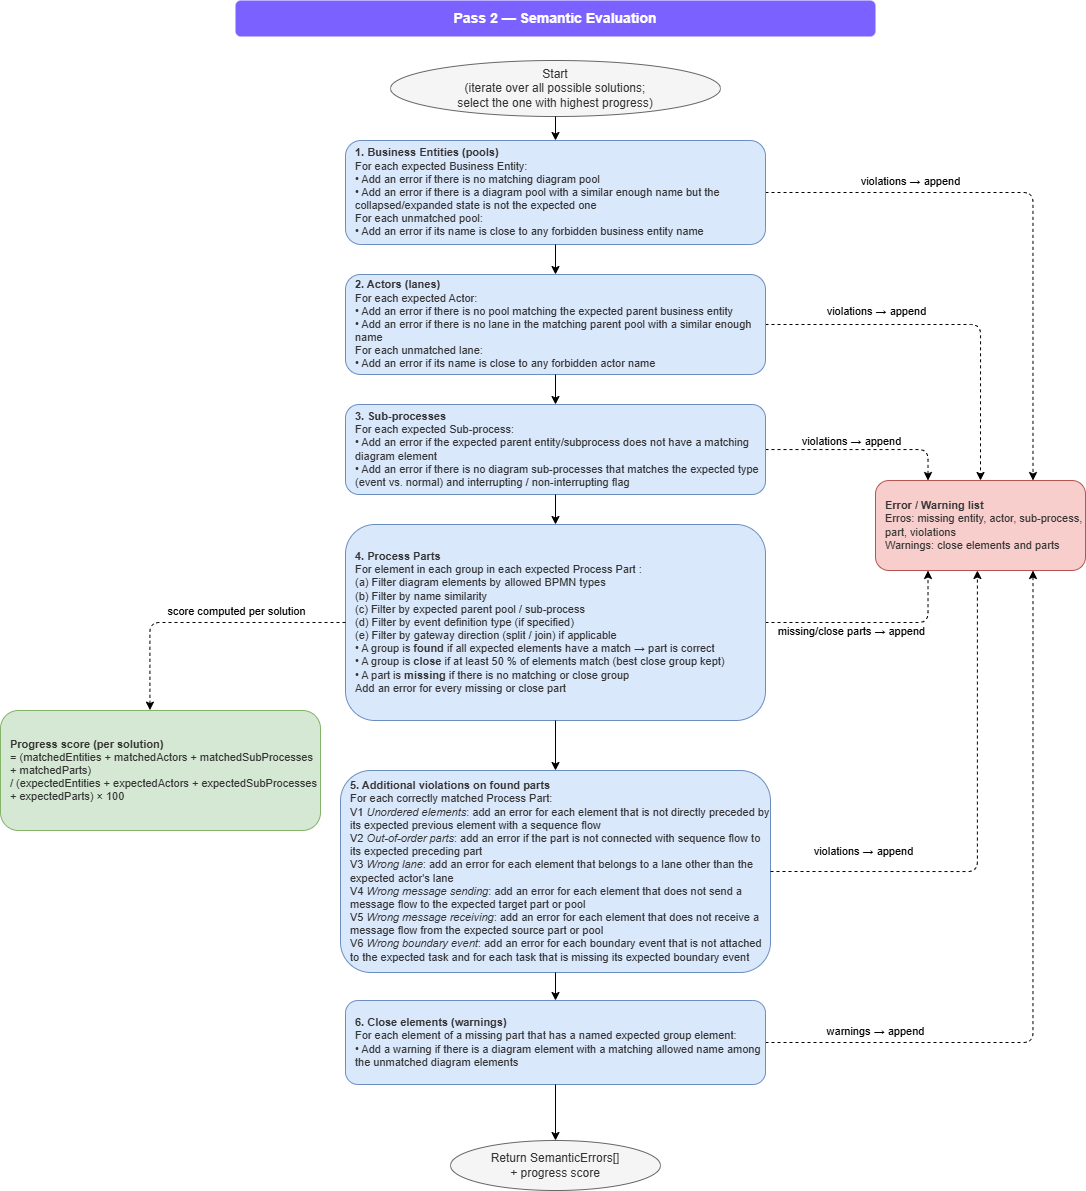
\includegraphics[width=0.75\linewidth]{Template_Latex_ScuDo_Tesi/Chapter5/sem_alg.png}
    \caption{Semantic evaluation algorithm}
    \label{fig:sem_alg_5}
\end{figure}

\subsection{Gamified Mechanics}

The implementation of the game mechanics for the new version of BIPMIN followed the same framework described in Chapter 4, distinguishing between long-term mechanics used to motivate continuous use of the application and exercise-specific ones that assist students when they perform their modeling assignments. Certain game mechanics were implemented with the same reasoning and behavior as in UMLegend, while others were adapted to the BPMN-specific context and with the goal of longitudinal use in mind; furthermore, two new exercise-specific mechanics were added, as well as a long-term one.

\textbf{Levels and Experience points} remained the key mechanic structured around showing a student's growth in modeling skill, and all experience management mechanics were implemented in the same way: errors would never reduce the obtainable experience below the minimum threshold of 35\%, multipliers for good performance when completing an exercise were kept, and the mechanism to recover experience when correcting errors was also put in place. Experience thresholds for leveling up, as well as obtainable experience points for exercise completion, were set to ensure that obtaining the minimum score in all exercises would be sufficient to reach the maximum level.  

\textbf{Avatar Customization} saw no change compared to the UMLegend implementation, keeping the original intention of using avatars as a way to let students customize their experience within the tool and its use in a course. In the context of a longitudinal use, certain avatar props were identified as rarer and set to be unlocked only at higher levels; in any case, all students who managed to complete all exercises would be able to obtain all avatar props.

\textbf{Leaderboards}, which were implemented in both the first prototype and in the UMLegend tool but had yet to show their potential as motivating elements saw the addition of a third leaderboard type, ranking students by the number of completed exercises. Additionally, since the goal was to use the BIPMIN tool in a classroom environment with a potentially high number of participants, it was decided to avoid using a single leaderboard showing all students using the tool but to introduce leaderboards showing the top 10 students for each ranking, and relative leaderboards showing students with a similar rank; this was done mainly to avoid potentially demotivating scenarios where students could perceive their ranking negatively compared to the large amount of colleagues.

A new long-term mechanic that was introduced aimed at building a sort of metaphor for the continuous challenge of solving increasingly harder exercises by adding the concept of enemies tied to the exercises in the form of stylized robotic bosses: a \textbf{Boss Icon} would appear inside each exercise, challenging the player with a message when starting an exercise and disappearing after completion, signifying the enemy's defeat. The boss icon does not appear only in the exercise interface but is also shown in the exercise's corresponding menu item in the home page after exercise completion, providing a visual feeling of reward and satisfaction.

Regarding exercise-dependent mechanics, most of them were changed with the exception of \textbf{Indicators}, \textbf{Avatar Feedback}, and the \textbf{In-exercise Leaderboard}, since their original interpretation had nothing specifically related to UML modeling or could benefit from changes based on longitudinal use.

For what concerns mechanics that were changed, instead \textbf{Error Lists} saw a relevant change with the removal of the list related to pragmatic warnings, since pragmatic quality for BPMN diagrams concerns mostly their readability, which cannot be easily assessed through automated element assessment, and the expansion of the shown messages so that, for each erroneous element, the BPMN source code identifier is listed with a detailed description, allowing for easy retrieval of the errors with the combination of the diagram feedback implementation and the \textit{bpmn.io} engine's support for element search through keyboard shortcuts.

\textbf{Process Parts Lists} were added as a new mechanic, with the same logic as the error-based lists: each correctly modeled process part would appear when clicking the list, showing the name of the matched part and the names and ids of the elements that satisfied the matching conditions; a similar reasoning was made for the list associated with close parts, where matching elements would be presented and the description of the missing elements were provided to guide students toward including the necessary process components. Lastly, the list for close elements was also added, stating for each element the description and the process part that said elements could be considered valid matches, and the reason behind the match not being complete (incorrect element type, belonging to the wrong pool, or both).

\textbf{Diagram Feedback} saw the most substantial change out of all game mechanics from the implementation used in the 2023 empirical study: rather than marking only elements that represented matched process parts by changing their color, multiple variations could be applied to various elements depending on the results of an automated evaluation. Certain icons could be added to elements depending on whether they were correct (a green check mark), close elements (a yellow exclamation mark), members of a close part (a yellow question mark), or in the wrong order within their process part or members of a part in the wrong order (a purple shuffle icon); other changes included changing the border of forbidden pools or names to red, changing the border of elements in the wrong lane to orange, changing the filling of message-based elements with no message flow to blue, and changing the border of elements that exchanged messages with the wrong elements to pink; the combination of all element changes and the feedback lists (where errors also shared the same color as the change in the diagram) ensured a better understanding of why certain modeling choices were considered correct, wrong, or incomplete but able to become correct with certain changes.

Lastly, \textbf{Exercise Hints} were added as a separate section inside an exercise's menu: these hints could be configured by a teacher when defining a reference solution and could be unlocked either as a reward for reaching certain completeness thresholds, to help students finalize almost complete diagrams, or as a catch-up mechanism after performing a high number of checks or losing enough experience.

An example of what an exercise's page looks like when the relevant mechanics are active can be seen in Figure \ref{fig:ex_page}, which shows a diagram with feedback highlighting errors and correct elements, the reaction of the student's avatar, the robotic enemy, and the completeness and experience indicators.

\begin{figure*}
    \centering
    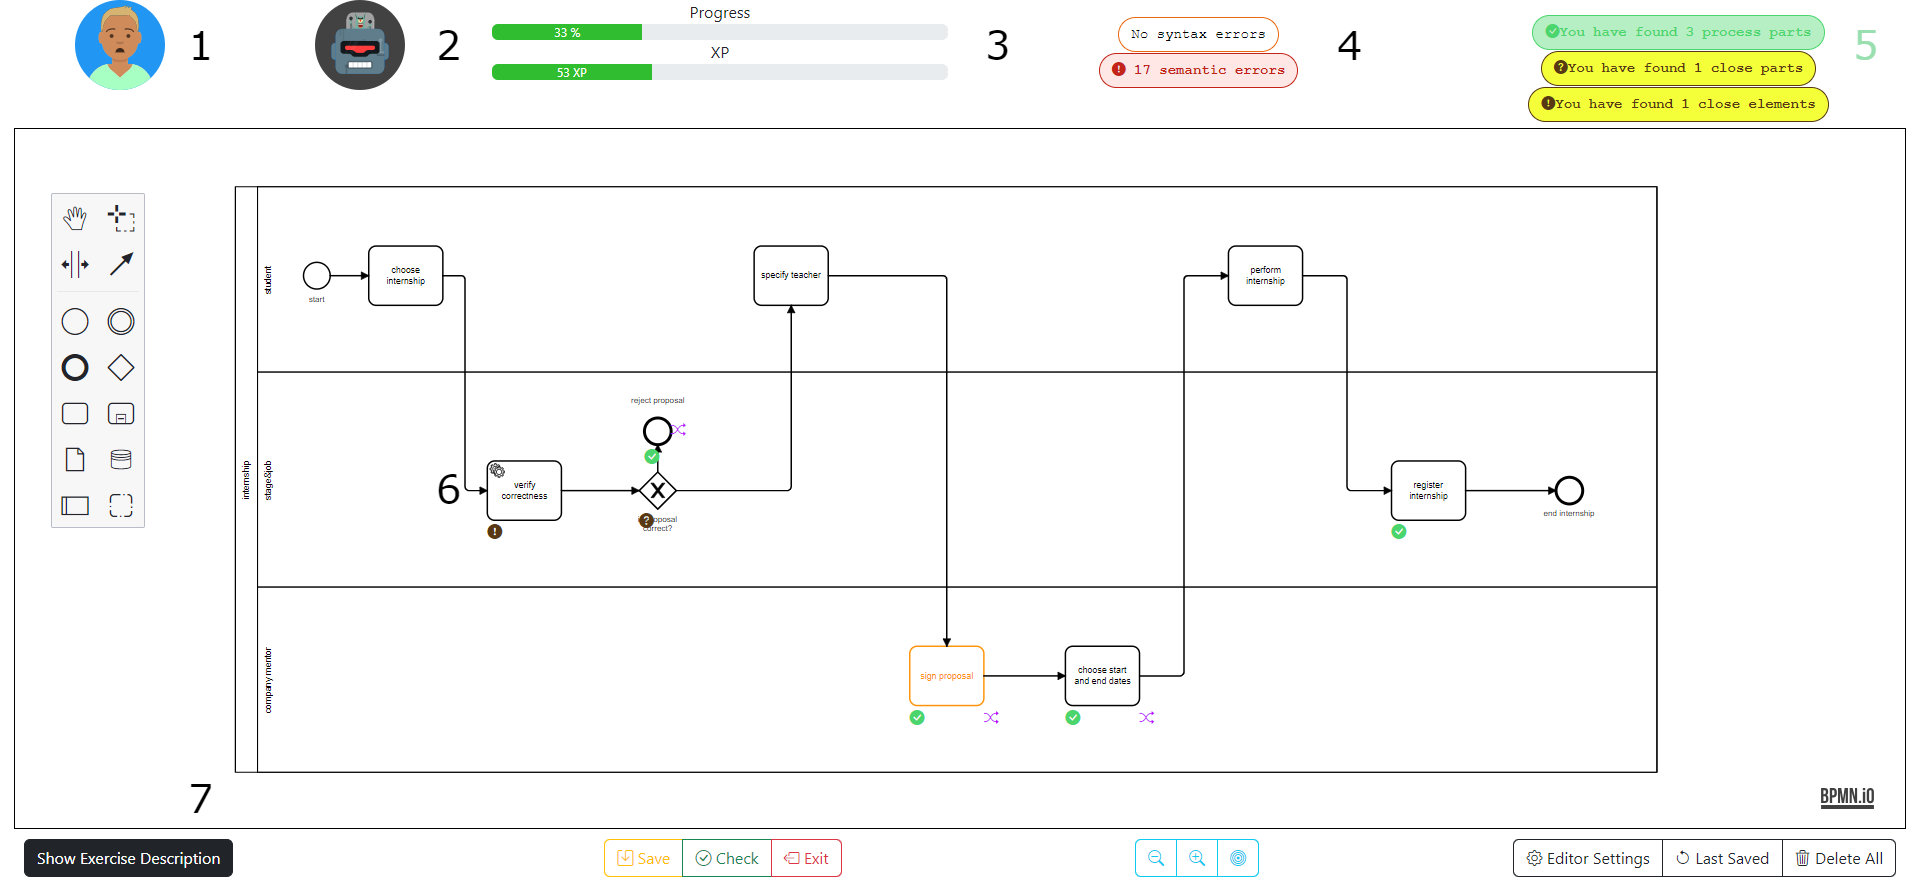
\includegraphics[width=0.9\linewidth]{Template_Latex_ScuDo_Tesi/Chapter5/ex_page.png}
    \caption{Exercise page in the revised BIPMIN application showing 1) Student Avatar, 2) Boss, 3) Indicator, 4) Error Lists, 5) Process Parts Lists, 6) Diagram Feedback, 7) Exercise Menu}
    \label{fig:ex_page}
\end{figure*}

\section{Longitudinal application of BIPMIN in an educational context}

The development of the improved version of BIPMIN was finalized by the beginning of October 2023, making it possible to deploy it for the 2023-2024 edition of the Information Systems course, the parallel English version of the course where UMLegend was later tested at the end of the course, allowing for two similar experiments within the same context: longitudinal effects of gamification on process modeling and comparison between regular and gamified-assisted UML modeling. 

BIPMIN was used during the entire course for practical BPMN modeling exercises, with five exercises of progressively increasing challenge level released throughout the course, starting from basic process flows and reaching advanced concepts such as event handling and communication between multiple pools. Students were encouraged to use the tool during practical lab lectures or on their own time, allowing for complete freedom of use with the only deadline for attempting exercises being the end of the course, to allow late-enrolling students participation as well.

To encourage participation, students were promised a reward of two additional points on their written exam's grade if they performed at least one attempt on each of the five exercises before the deadline, requiring at least a minimum level of effort (e.g., not submitting empty diagrams or diagrams solved randomly) as the only constraints needed to obtain the reward; completing exercises by obtaining the minimum completeness threshold was not added as a condition for the reward to ensure students would not be discouraged in case of performance they felt was unsatisfactory. 

Activities outside of the lab exercises such as theory lectures or the group-based project work were, however, performed using the same platform used in past years, since it offered collaborative features that were not yet implemented in BIPMIN, leading to practical BPMN exercises being the only course topic done with a gamified approach.

Out of 363 students enrolled in the course, 264 performed at least one exercise, with 254 students trying all five at least once; 200 students passed the exam by the end of the winter exam session and were considered for the analysis on the educational impact. A final questionnaire was provided in the final week of the course to collect the students' opinions and suggestions related to their experience with the tool; 248 students who used the tool at least once answered all questions.


\section{Empirical evaluation of the long-term usage}

The experiment focused on the longitudinal use of BIPMIN started in October 2023 and was finalized at the end of January 2024, following the end of the course and the subsequent exam session, where it was possible to observe the effects of gamification on the students' acquired BPMN modeling skills. The experimental design was planned at the start of the course following, in the same vein as the 2023 empirical study, according to the GQM template; Table \ref{tab:gqm5} summarizes the experiment's research objectives, while the purpose of the study was formalized as \textit{assess the impact of the longitudinal adoption of gamification on learning BPMN modeling from the point of view of Software Engineering teachers in the context of university courses}.

\begin{table}[ht]
\centering
\caption{GQM template for the experiment}
\label{tab:gqm5}
\footnotesize
\begin{tabular}{@{}p{0.3\columnwidth} p{0.55\columnwidth}@{}}
\toprule
Object of Study & Learning of BPMN Modeling \\
Purpose & Assess the impact of gamification \\
Focus & Grades, Learning Progress, Commitment  \\
Context & Modeling tools, Education \\
Perspective & Teachers, Learners\\
\bottomrule
\end{tabular}
\end{table}

\subsection{Research Questions and Metrics}

The study was designed to answer the following research questions:

\begin{itemize}
    \item[\textbf{RQ1}] Effectiveness: does gamification affect grades?\\
    \textit{The goal of this question is to observe whether long-term exposure to gamified BPMN modeling can have a positive effect on the students' grades.}
    This question is further refined into:
    \begin{itemize}
        \item[\textbf{RQ1.1}] Does the application of gamification impact the students’ grades in BPMN exercises for the final exam of the course?
        \item[\textbf{RQ1.2:}] Does the application of gamification impact the students' grades in BPMN exercises for the end-of-course project work?
    \end{itemize}
    \item[\textbf{RQ2}] Progress: does gamification support progressive learning during the course?\\
    \emph{The expectation is that gamification should support the incremental acquisition of modeling skills leading to progressively increasing quality of produced models.}\\
    This question is further refined into:
    \begin{itemize}
        \item[\textbf{RQ2.1:}] Does the application of gamification impact the correctness of the students' exercises during the course?
        \item[\textbf{RQ2.2:}] Does the application of  gamification impact the errors made by the students throughout the course?
        \item[\textbf{RQ2.3:}] Does the application of  gamification impact the completion rate of the exercises?
    \end{itemize}
    \item[\textbf{RQ3}] Perception: is gamification well received by the students?\\
    \emph{The assumption behind this question is that gamification will be positively perceived by the students with more involvement and willingness to adopt it.}\\
    This question is further refined into:
    \begin{itemize}
        \item[\textbf{RQ3.1:}] What is the perceived usability of the BIPMIN application?
        \item[\textbf{RQ3.2:}] What is the students' appreciation of the BIPMIN tool?
        \item[\textbf{RQ3.3}:] What are the students' opinions related to the longitudinal use of BIPMIN?
    \end{itemize}
\end{itemize}

The comparison between the regular BPMN learning approach and gamification-enhanced one was selected as the strategy to answer RQ1: the intention was to observe how the students who used BIPMIN throughout the course performed in the final BPMN-related assignments and assess differences with grades obtained by students who followed a traditional learning approach. For this purpose, grades obtained by students enrolled in the 2022/2023 edition of the course were retrieved and compared with the ones obtained by participants in the longitudinal study: the independent variable considered for answering RQ1 was set as the academic year, while two dependent variables were analyzed, the points obtained in the BPMN exercises of the final exam, ranging from a minimum of 0 and a maximum of 8 and testing theoretical knowledge of BPMN fundamentals and ability to discern correct modeling choices, and the grade assigned to the BPMN part of the end-of course project work, which tested the students' ability to represent complex processes involving multiple entities, actors and requirements with a score interval of 0 to 5.

RQ2, instead, followed a different approach: the goal of the question was to measure the students' learning progression over time, with five total exercises made available for completion over the course's duration: exercises were selected to introduce a progressive challenge with increasing difficulty levels, making it possible to observe the students' growth in modeling skill; consequently, the exercise number was chosen as the independent variable for answering RQ2, and dependent variables were three metrics computed directly by the tool for each exercise (the exercise completeness computed as the sum of matched elements over the total set of expected elements and the counts of both syntax and semantic errors).   

The method used to answer RQ3 and its sub-questions followed the same approach used for the UMLegend study: the final questionnaire was structured in a very similar way, with questions taken from the TAM \cite{davis1989perceived, lee2003technology} and GAMEX \cite{eppmann2018gameful} questionnaires used to assess the overall perception of the tool's usability and of the gamified experience, allowing answers through a Likert scale from 1 to 5 and providing a way to answer RQ3.1.

Questions focused on the game mechanics were also included to answer RQ3.2, with additional questions for the new mechanics implemented specifically in BIPMIN, as well as questions related specifically to the longitudinal experience and how students perceived the impact of the long-term use of the tool in term of learning, asking about the effects on improving their modeling skills, on learning BPMN fundamental rules, on fixing errors, and on the negative effects such as distractions during the course. These additional questions were also structured with a 1-5 Likert scale for the answers.

Finally, two open questions were included as the way to answer RQ3.3, asking students about their suggestions on improvement areas for the tool and on how to better integrate BIPMIN in the general course execution.

\subsection{Analysis Method}

A total of five null hypotheses were formulated to frame the study, with two hypotheses for RQ1 and three for RQ2; these hypotheses are as follows:


\begin{itemize}
    \item \textbf{${H_{1.1_{0}}}$:} The application of gamification has no statistically significant impact on the grade obtained by students for the BPMN-related exercises of the final written exam;
    \item \textbf{${H_{1.2_{0}}}$:} The application of gamification has no statistically significant impact on the grade obtained by students for the BPMN-related exercises of the end-of-course project work;
    \item \textbf{${H_{2.1_{0}}}$:} The application of gamification does not lead to a statistically significant improvement in the completeness score obtained in the exercises throughout the course;
    \item \textbf{${H_{2.2_{0}}}$:} The application of gamification does not lead to a statistically significant reduction in the number of syntax errors made in the exercises throughout the course;
    \item \textbf{${H_{2.3_{0}}}$:} The application of gamification does not lead to a statistically significant reduction in the number of semantic errors made in the exercises throughout the course.
\end{itemize}

Two different analysis approaches were performed depending on the research question: to evaluate hypotheses associated with RQ1, a Wilcoxon test was conducted on the distribution of the two grade metrics using the academic year as the independent variable. RQ2 hypotheses, instead, were evaluated with two distinct encoding methods: first, a fixed effects linear model analysis was performed by taking the first exercise as the reference level and assessing differences in scores obtained in the following four exercises; then a linear model with a progressive reference, allowing for a comparison between each exercise and the following one. The purpose of both methods was to observe trends in modeling performance in comparison with the start of the course, to identify potential positive effects over time, as well as comparing relative progression in consecutive exercises, to identify the students' ability to assimilate complex topics.

Given the fact that multiple univariate tests were performed, to counteract the risk of increasing the chance of false positives and have Type I errors, the significance level was adjusted by applying Bonferroni correction, resulting in a new p-value threshold of $\alpha_C = \alpha / 8 =  0.00625$ to identify statistical significance. The eight independent tests come from the fact that each RQ2 hypothesis is tested using two linear-model encodings, derived from the count of 2 (RQ1 metrics with a single test each) + 3 (RQ2 metrics) x 2 (tests).

The analysis of the questionnaire's answers was performed with the same approach used for the two empirical studies described in Chapters 3 and 4: answers given to Likert-based questions were grouped by questionnaire construct (e.g., TAM or GAMEX measure, game mechanic) and the resulting average taken as the general opinion for each student, leading to the distribution of opinions showing the participants' interpretation of the experience.

Answers to the two open questions were instead analyzed with an \textit{open coding} approach (see Section \ref{sec:empirical_methods})\cite{strauss1998basics} with a two-iteration procedure: after identifying topics across all answers, answers were analyzed again to identify a potentially more relevant topic to assign them out of the set. 

\subsection{Results}

Table \ref{tab:rq1_5} summarizes the statistics related to the RQ1 metrics, the grade obtained in BPMN tasks in the final written exam and the one obtained in the BPMN assignment of the end of course project, divided per academic year, with 2023 being the year where non-gamified BPMN teaching methods were used, and 2024 being the academic year where BIPMIN was adopted for practical assignments. The distribution of both metrics according to the academic year is shown in Figure \ref{fig:rq1_5}.

\begin{table}[ht]
    \footnotesize
    \centering
    \caption{Summary statistics (minimum, maximum, mean, median, standard deviation) for Effectiveness metrics}
    \begin{tabular}{llrrrr}
    \toprule
    Type & Year & Min & Max & Mean (SD) & Median \\
    \midrule
    Exam Grade & 2023 & 0.0 & 8 & 5.83 (1.65) & 6.30 \\
    Exam Grade & 2024 & 1.6 & 8 & 6.56 (1.78) & 7.00 \\
    Project Grade & 2023 & 0.0 & 5 & 2.05 (1.20) & 2.33 \\
    Project Grade & 2024 & 2.5 & 5 & 4.45 (0.56) & 4.50 \\
    \bottomrule
    \end{tabular}
    \label{tab:rq1_5}
\end{table}

\begin{figure}[H]
    \centering
    \begin{subfigure}{0.48\linewidth}
        \centering
        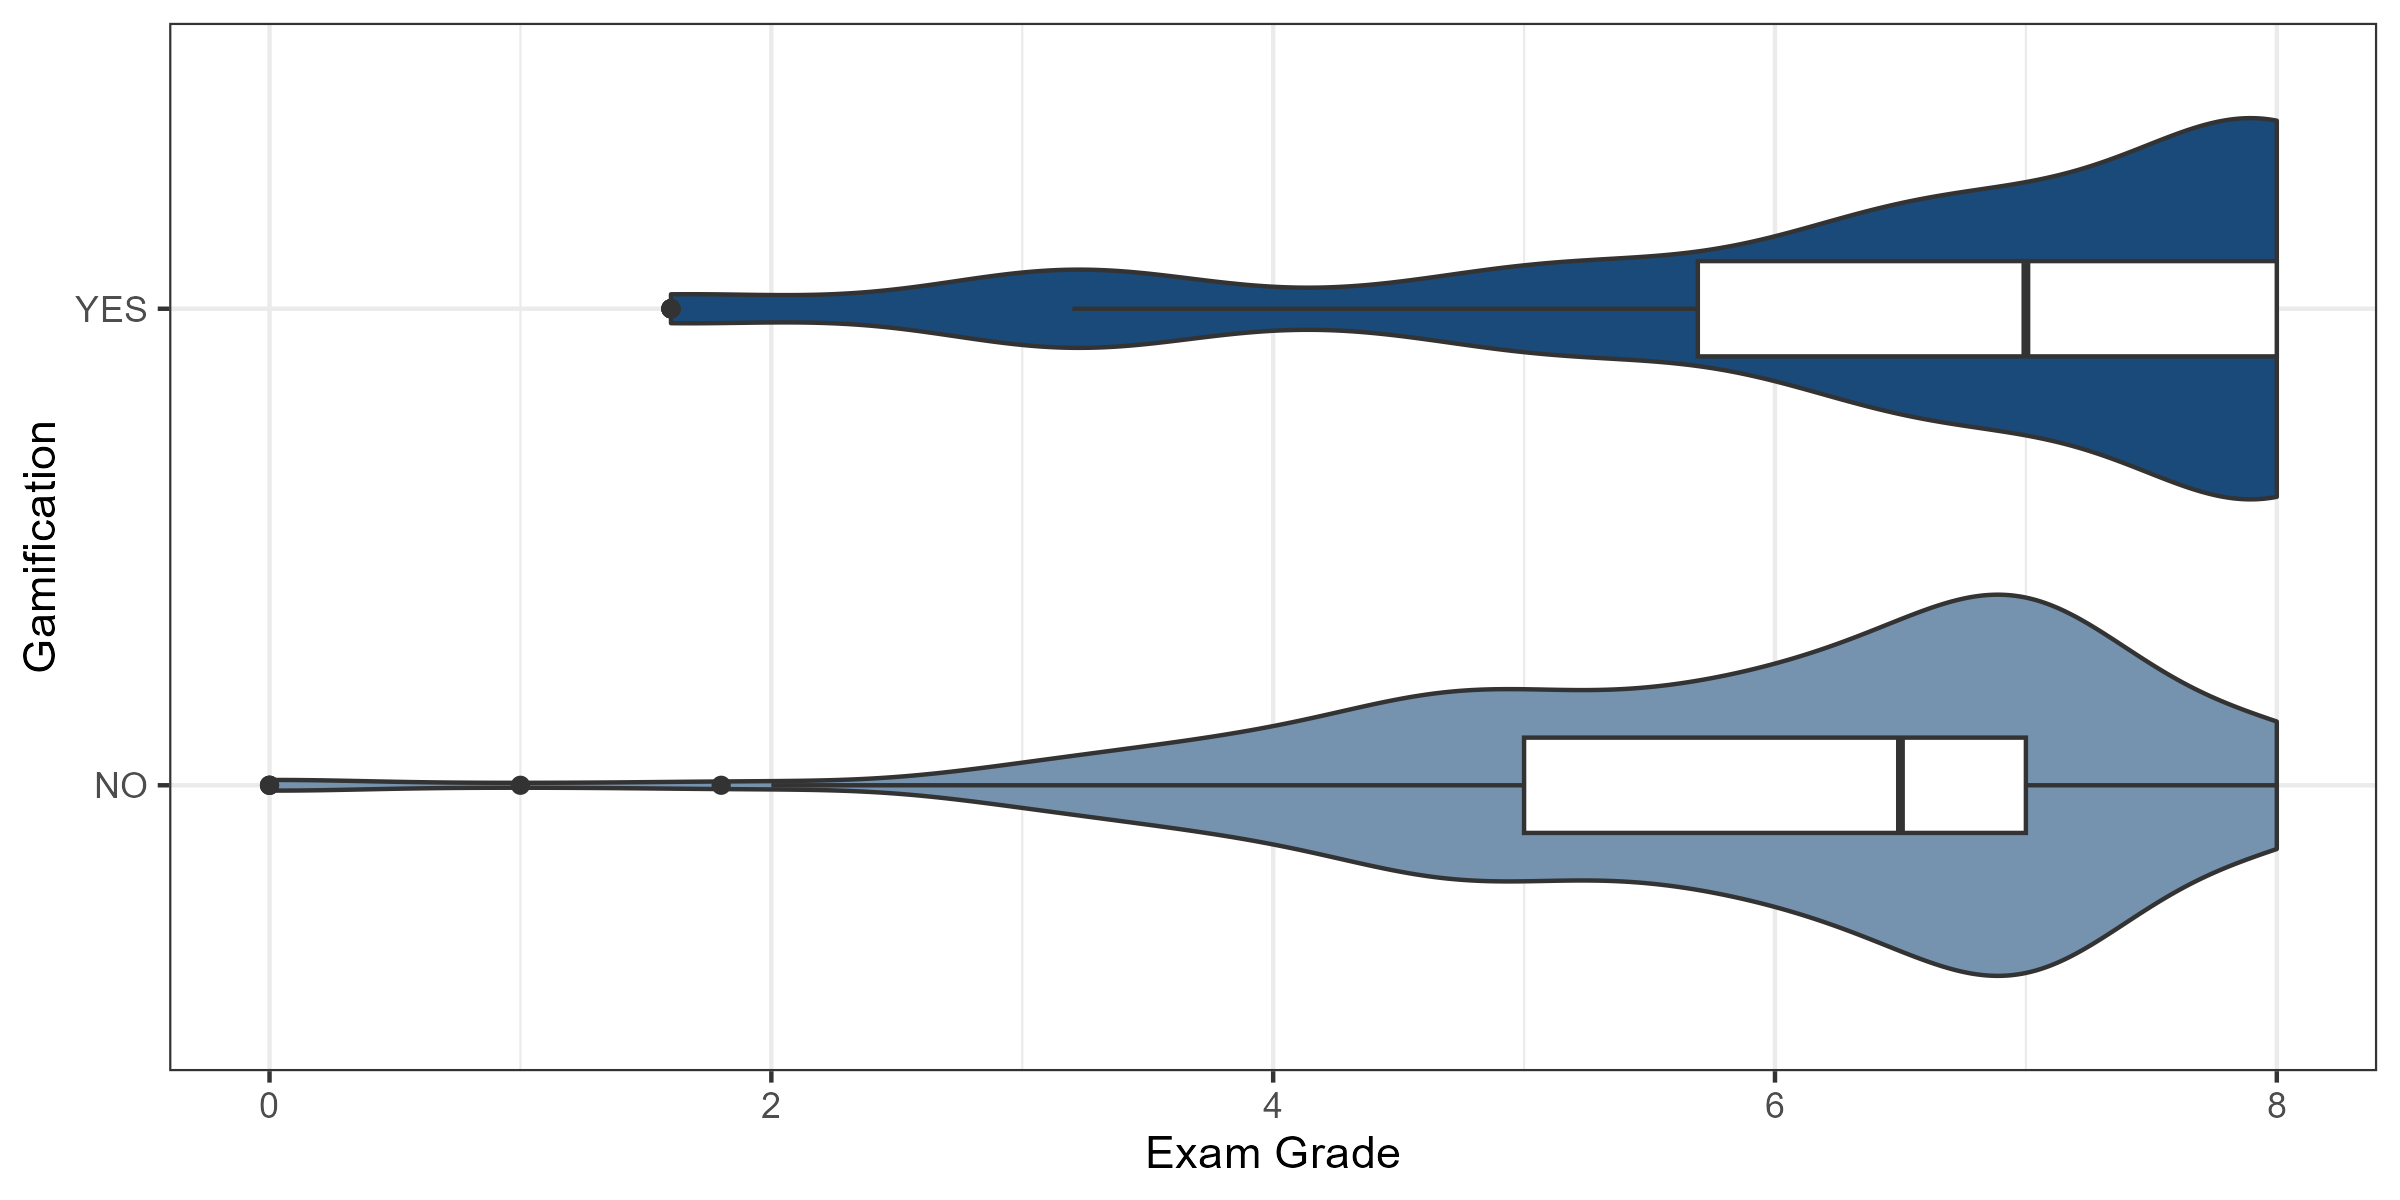
\includegraphics[width=\linewidth]{Template_Latex_ScuDo_Tesi/Chapter5/exam_violin.png}
        \caption{Box and violin plot for the distribution of exam grades for BPMN tasks}
        \label{fig:rq1_5_exam}
    \end{subfigure}\hfill
    \begin{subfigure}{0.48\linewidth}
        \centering
        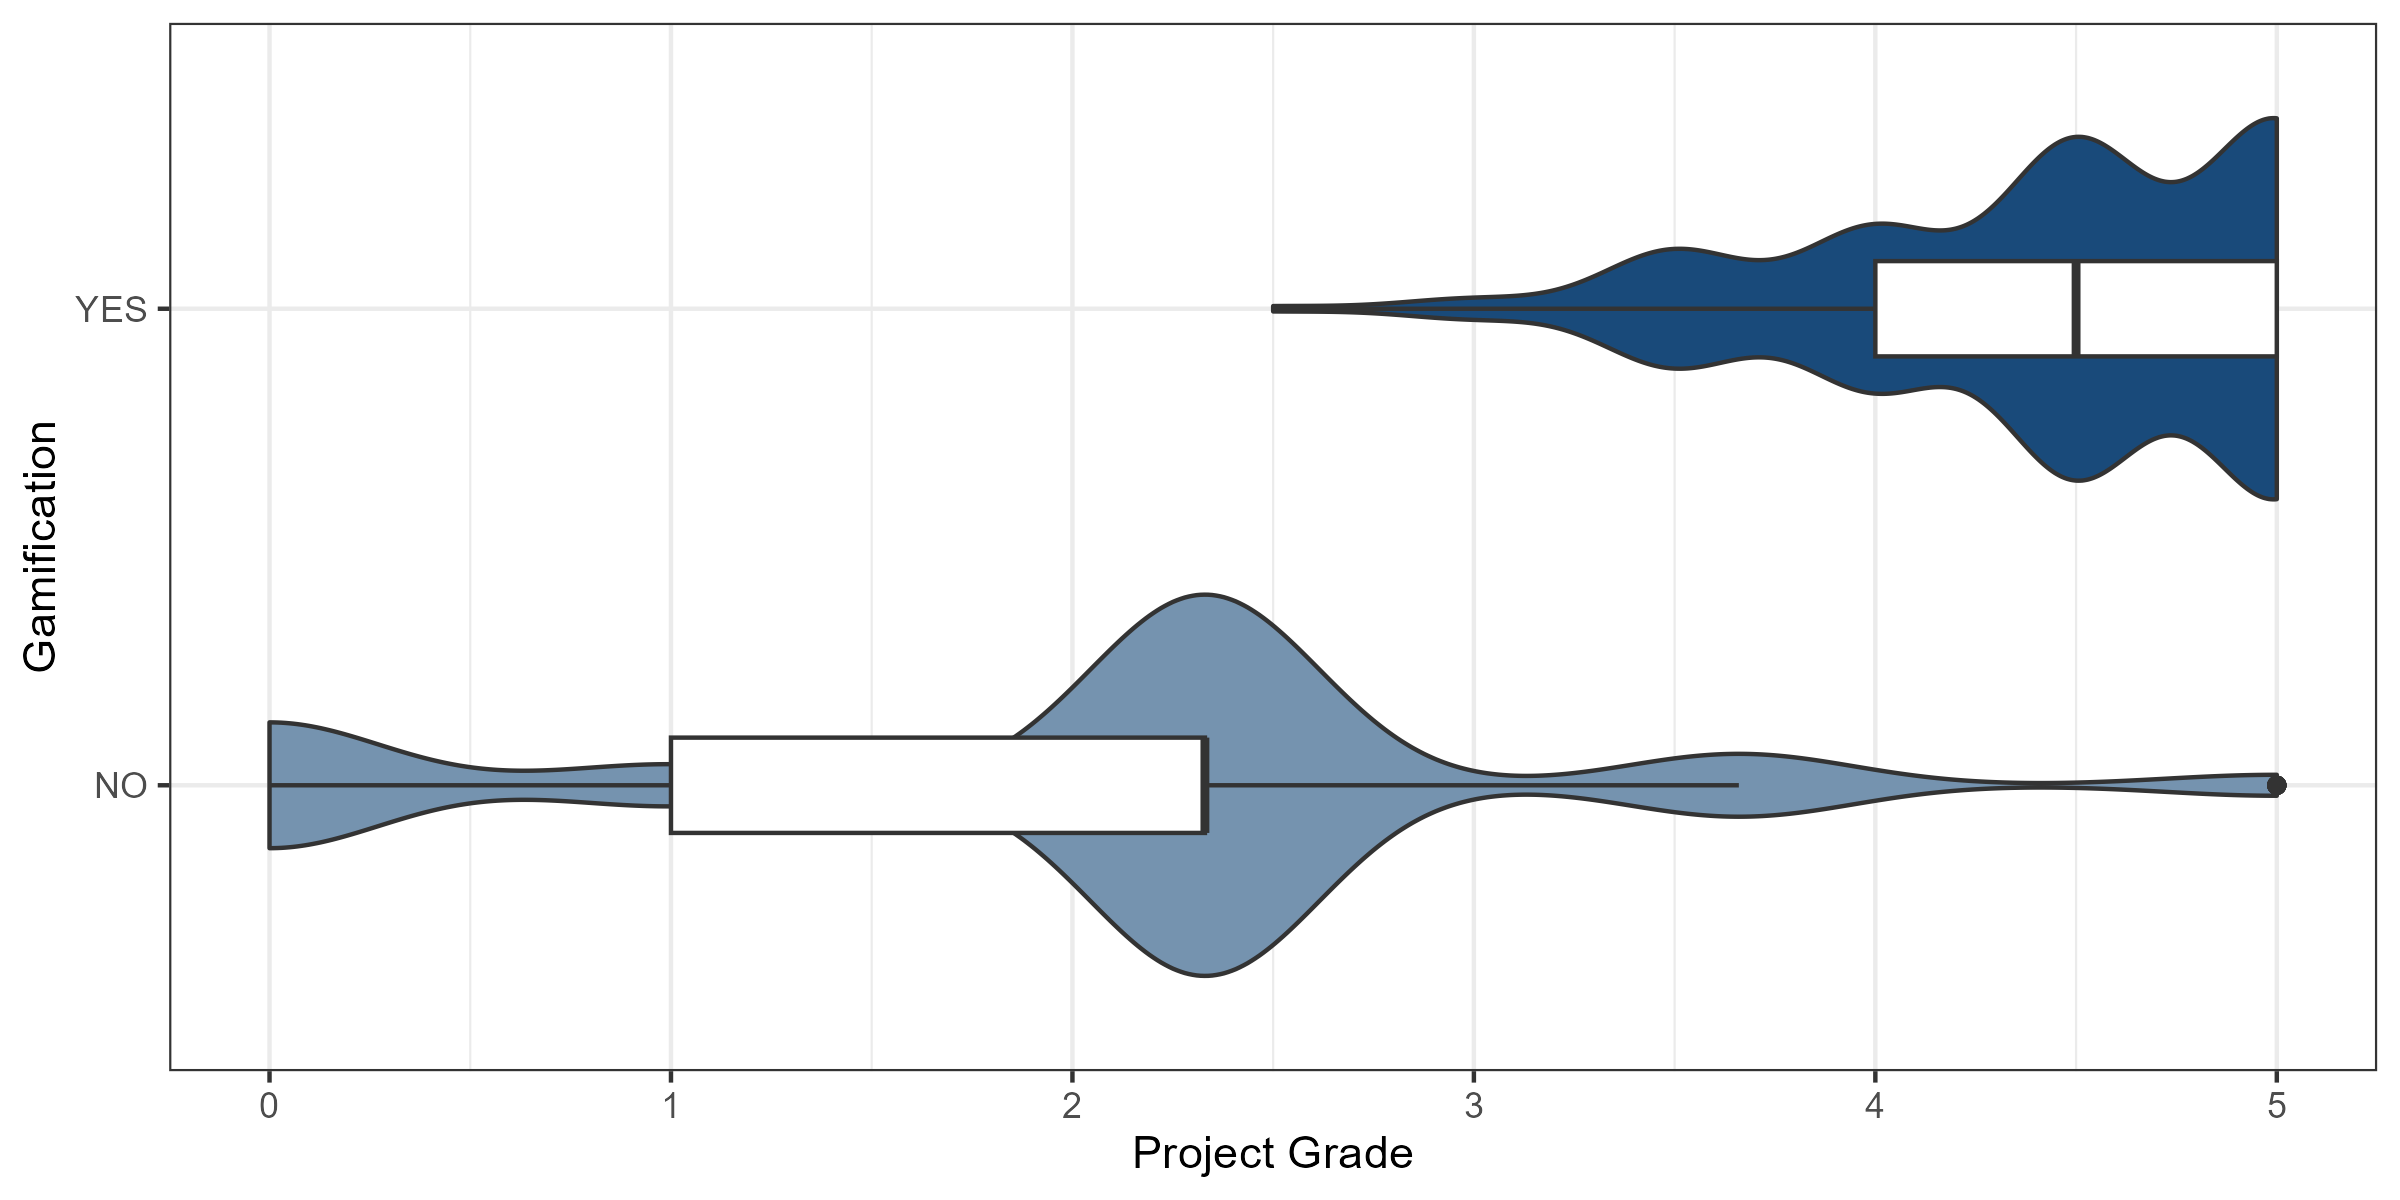
\includegraphics[width=\linewidth]{Template_Latex_ScuDo_Tesi/Chapter5/proj_violin.png}
        \caption{Box and violin plot for the distribution of grades for the project work's BPMN assignments}
        \label{fig:rq1__5_proj}
    \end{subfigure}
    \caption{Box and violin plots for RQ1 metrics}
    \label{fig:rq1_5}
\end{figure}

For both metrics, it is immediately obvious that performance was on average better in the 2024 edition of the course, with an increase of 11\% for exam scores and of 54\% for project scores, implying a potential positive effect of gamification on learning effectiveness. To answer RQ1, two Wilcoxon tests have been performed on both metrics, yielding a p-value of 1.09e-08 for exam grades: this value is statistically significant, making it possible to reject hypothesis ${H_{1.1_{0}}}$. Similarly, the test on project grades obtained a statistically significant p-value (p = \textless{} 2.2e-16), meaning that ${H_{1.2_{0}}}$ can also be rejected.

\answer{RQ1}{The longitudinal use of a gamified environment to teach BPMN modeling had a statistically significant effect on student grades, leading to an increase in both exam and project grades. It is reasonable to assume that using BIPMIN helped students improve their theoretical understanding of BPMN and their ability to identify correct modeling decisions, skills that are measured with the exam tasks, as well as their ability to handle complex processes based on real-life enterprise applications, which are the target of the project work.}

Regarding RQ2, diagram completeness and both syntax and semantic error counts were taken at the end of the course through BIPMIN's admin interface, considering, for each student, the values of the three metrics associated with their last saved diagram, assuming those to be their final scores; Table \ref{tab:rq2_5} presents minimum, maximum, mean, median, and standard deviation of the three metrics, while their distribution per exercise can be seen in Figure \ref{fig:rq2_5}.

\begin{table}[ht]
    \footnotesize
    \centering
    \caption{Summary statistics (minimum, maximum, mean, median, standard deviation) for Learning Progress metrics}
    \begin{tabular}{llrrrrr}
    \toprule
    Exercise & Metric & Min & Max & Mean (SD) & Median \\
    \midrule
    1 & Completeness         &  0 & 100 & 76.32 (21.73) & 82.00 \\
    1 & Syntax Errors    &  0 &  23 &  1.08 (2.55)  &  0.00 \\
    1 & Semantic Errors  &  0 &  23 &  8.04 (4.88)  &  7.00 \\
    \midrule
    2 & Completeness        &  0 & 100 & 71.95 (20.99) & 77.00 \\
    2 & Syntax Errors    &  0 &  21 &  0.71 (2.18)  &  0.00 \\
    2 & Semantic Errors  &  0 &  18 &  7.11 (4.19)  &  7.00 \\
    \midrule
    3 & Completeness         &  0 & 100 & 77.39 (21.33) & 85.00 \\
    3 & Syntax Errors    &  0 &  15 &  0.57 (1.47)  &  0.00 \\
    3 & Semantic Errors  &  0 &   9 &  4.42 (2.56)  &  5.00 \\
    \midrule
    4 & Completeness         &  0 & 100 & 77.45 (19.07) & 80.00 \\
    4 & Syntax Errors    &  0 &  12 &  1.44 (2.53)  &  0.00 \\
    4 & Semantic Errors  &  0 &  18 &  5.78 (4.12)  &  5.00 \\
    \midrule
    5 & Completeness         &  9 & 100 & 78.72 (19.64) & 84.00 \\
    5 & Syntax Errors    &  0 &  27 &  1.24 (2.92)  &  0.00 \\
    5 & Semantic Errors  &  0 &  14 &  5.64 (3.54)  &  5.00 \\
    \bottomrule
    \end{tabular}
    \label{tab:rq2_5}
\end{table}


\begin{figure}[H]
    \centering
    \begin{subfigure}{0.6\linewidth}
        \centering
        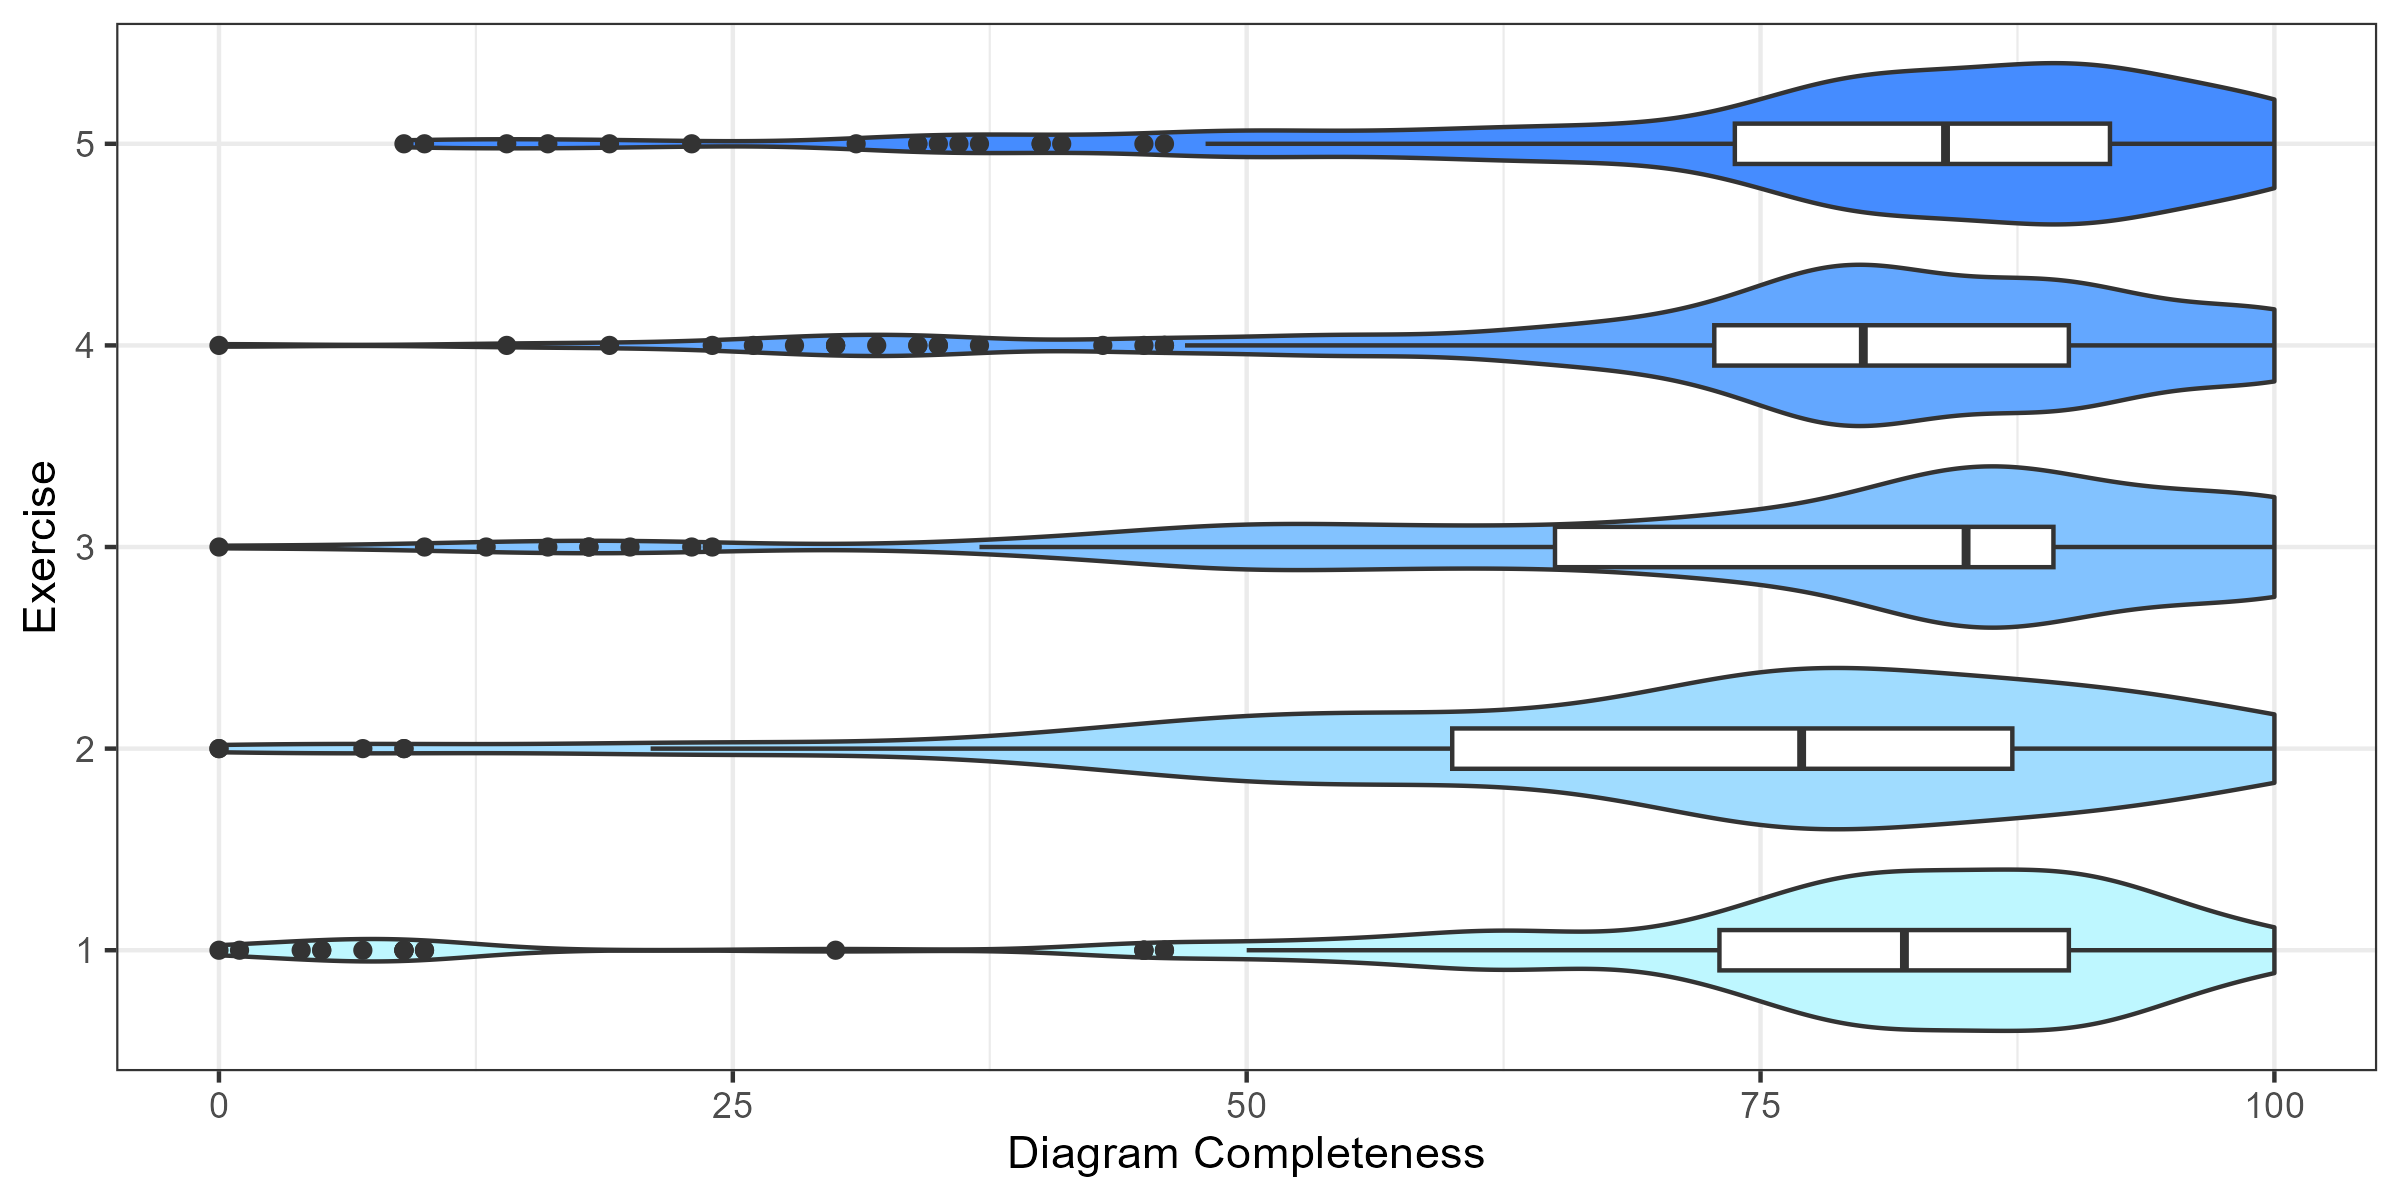
\includegraphics[width=\linewidth]{Template_Latex_ScuDo_Tesi/Chapter5/prog_violin.png}
        \caption{Box and violin plot for the distribution of diagram completeness per exercise}
        \label{fig:rq2_5_comp}
    \end{subfigure}\hfill
    \begin{subfigure}{0.6\linewidth}
        \centering
        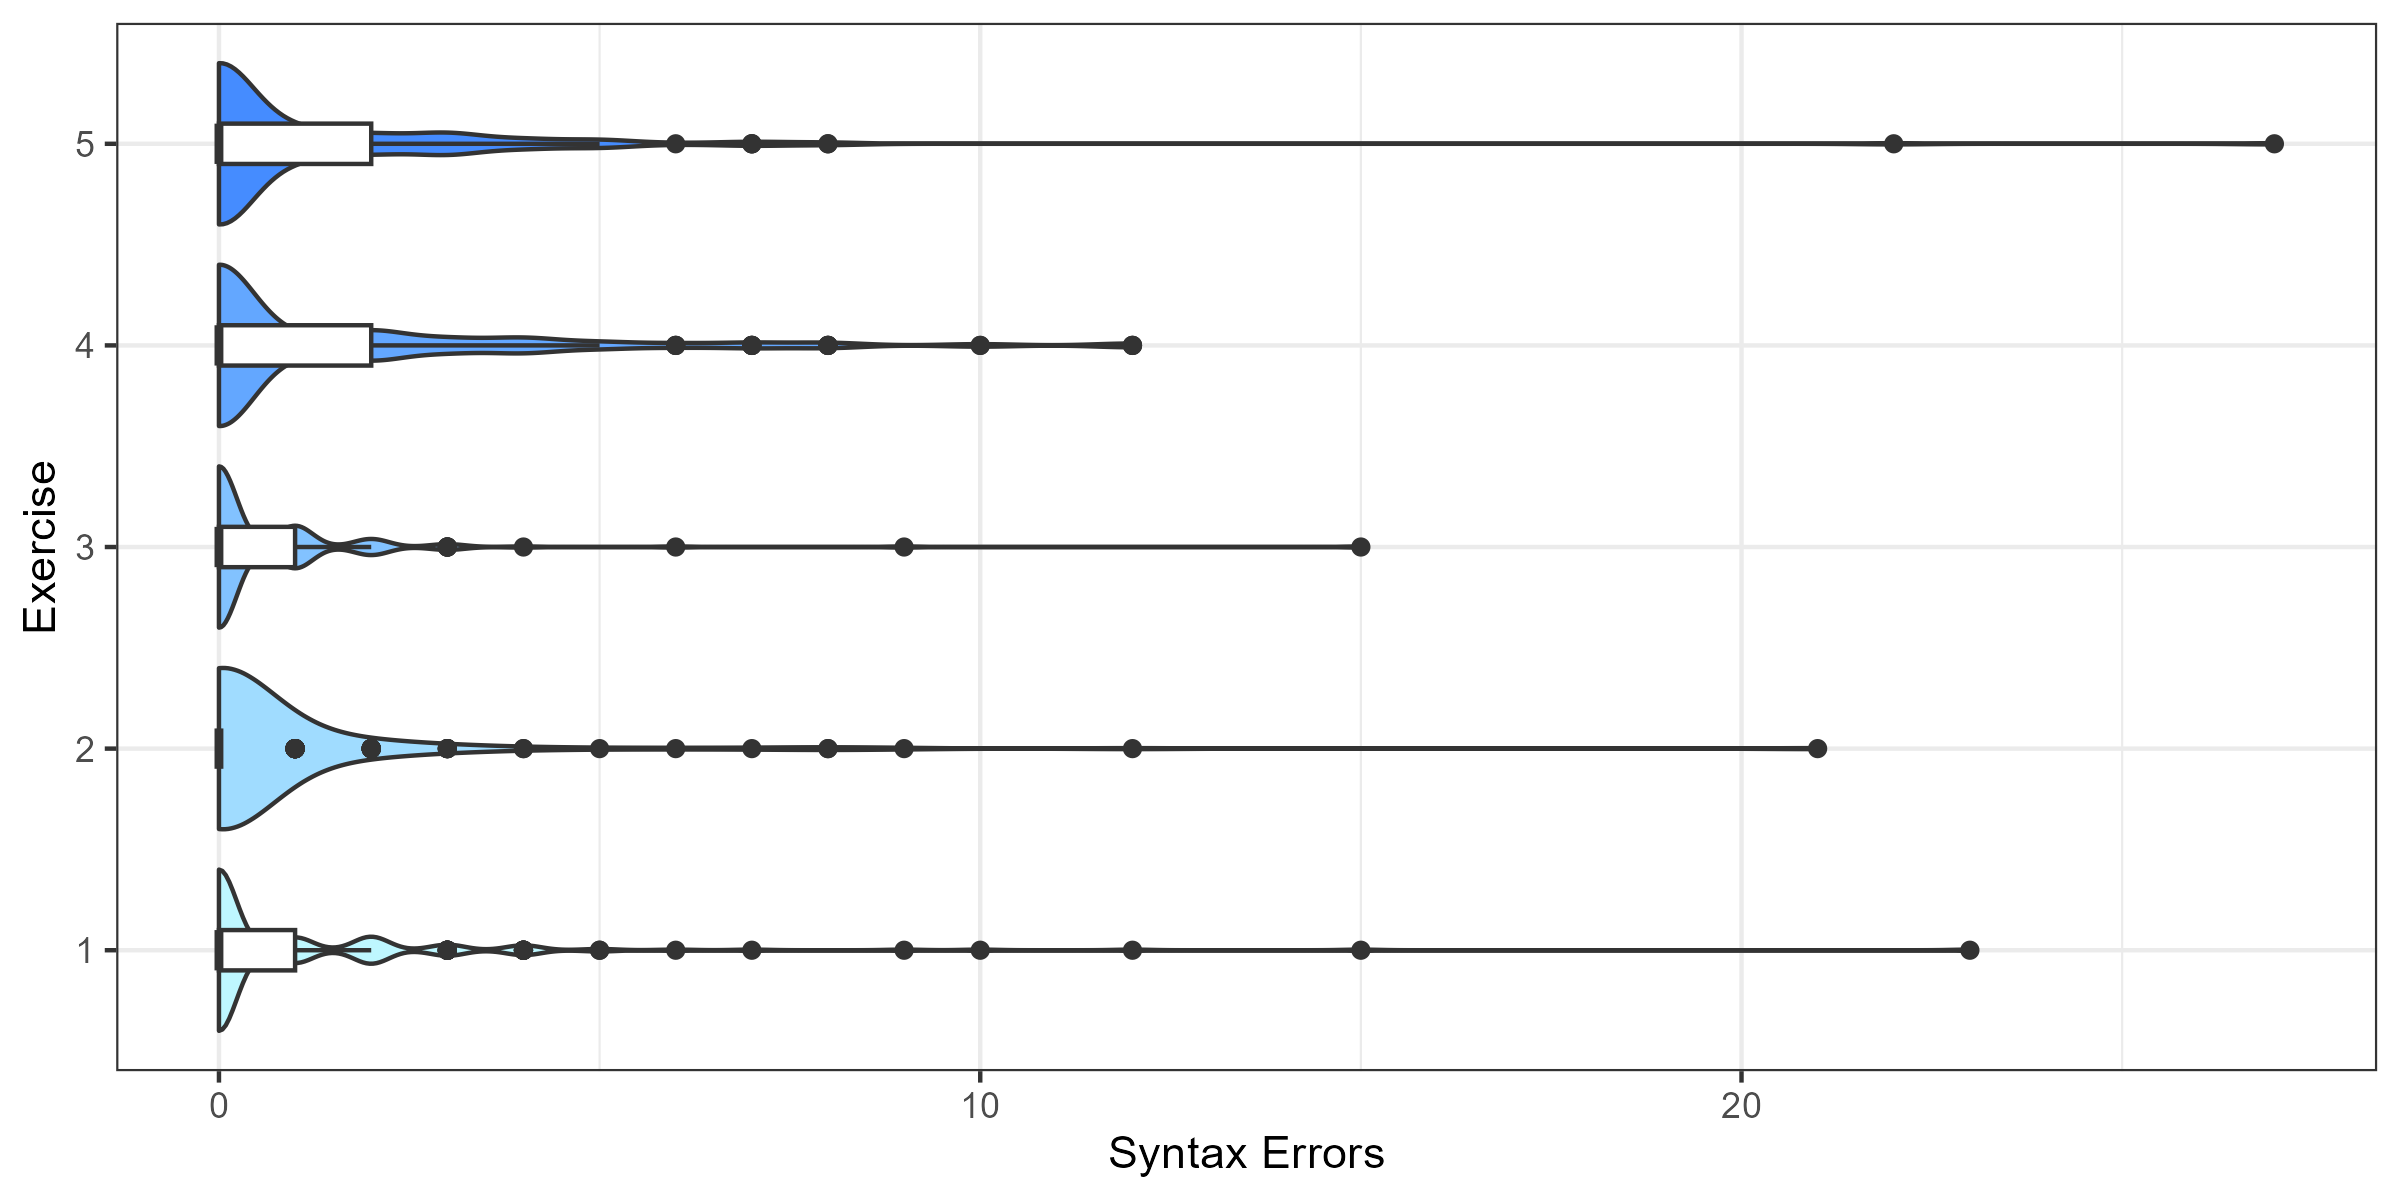
\includegraphics[width=\linewidth]{Template_Latex_ScuDo_Tesi/Chapter5/syn_violin.png}
        \caption{Box and violin plot for the distribution of syntax error counts per exercise}
        \label{fig:rq2_5_syn}
    \end{subfigure}\hfill
    \begin{subfigure}{0.6\linewidth}
        \centering
        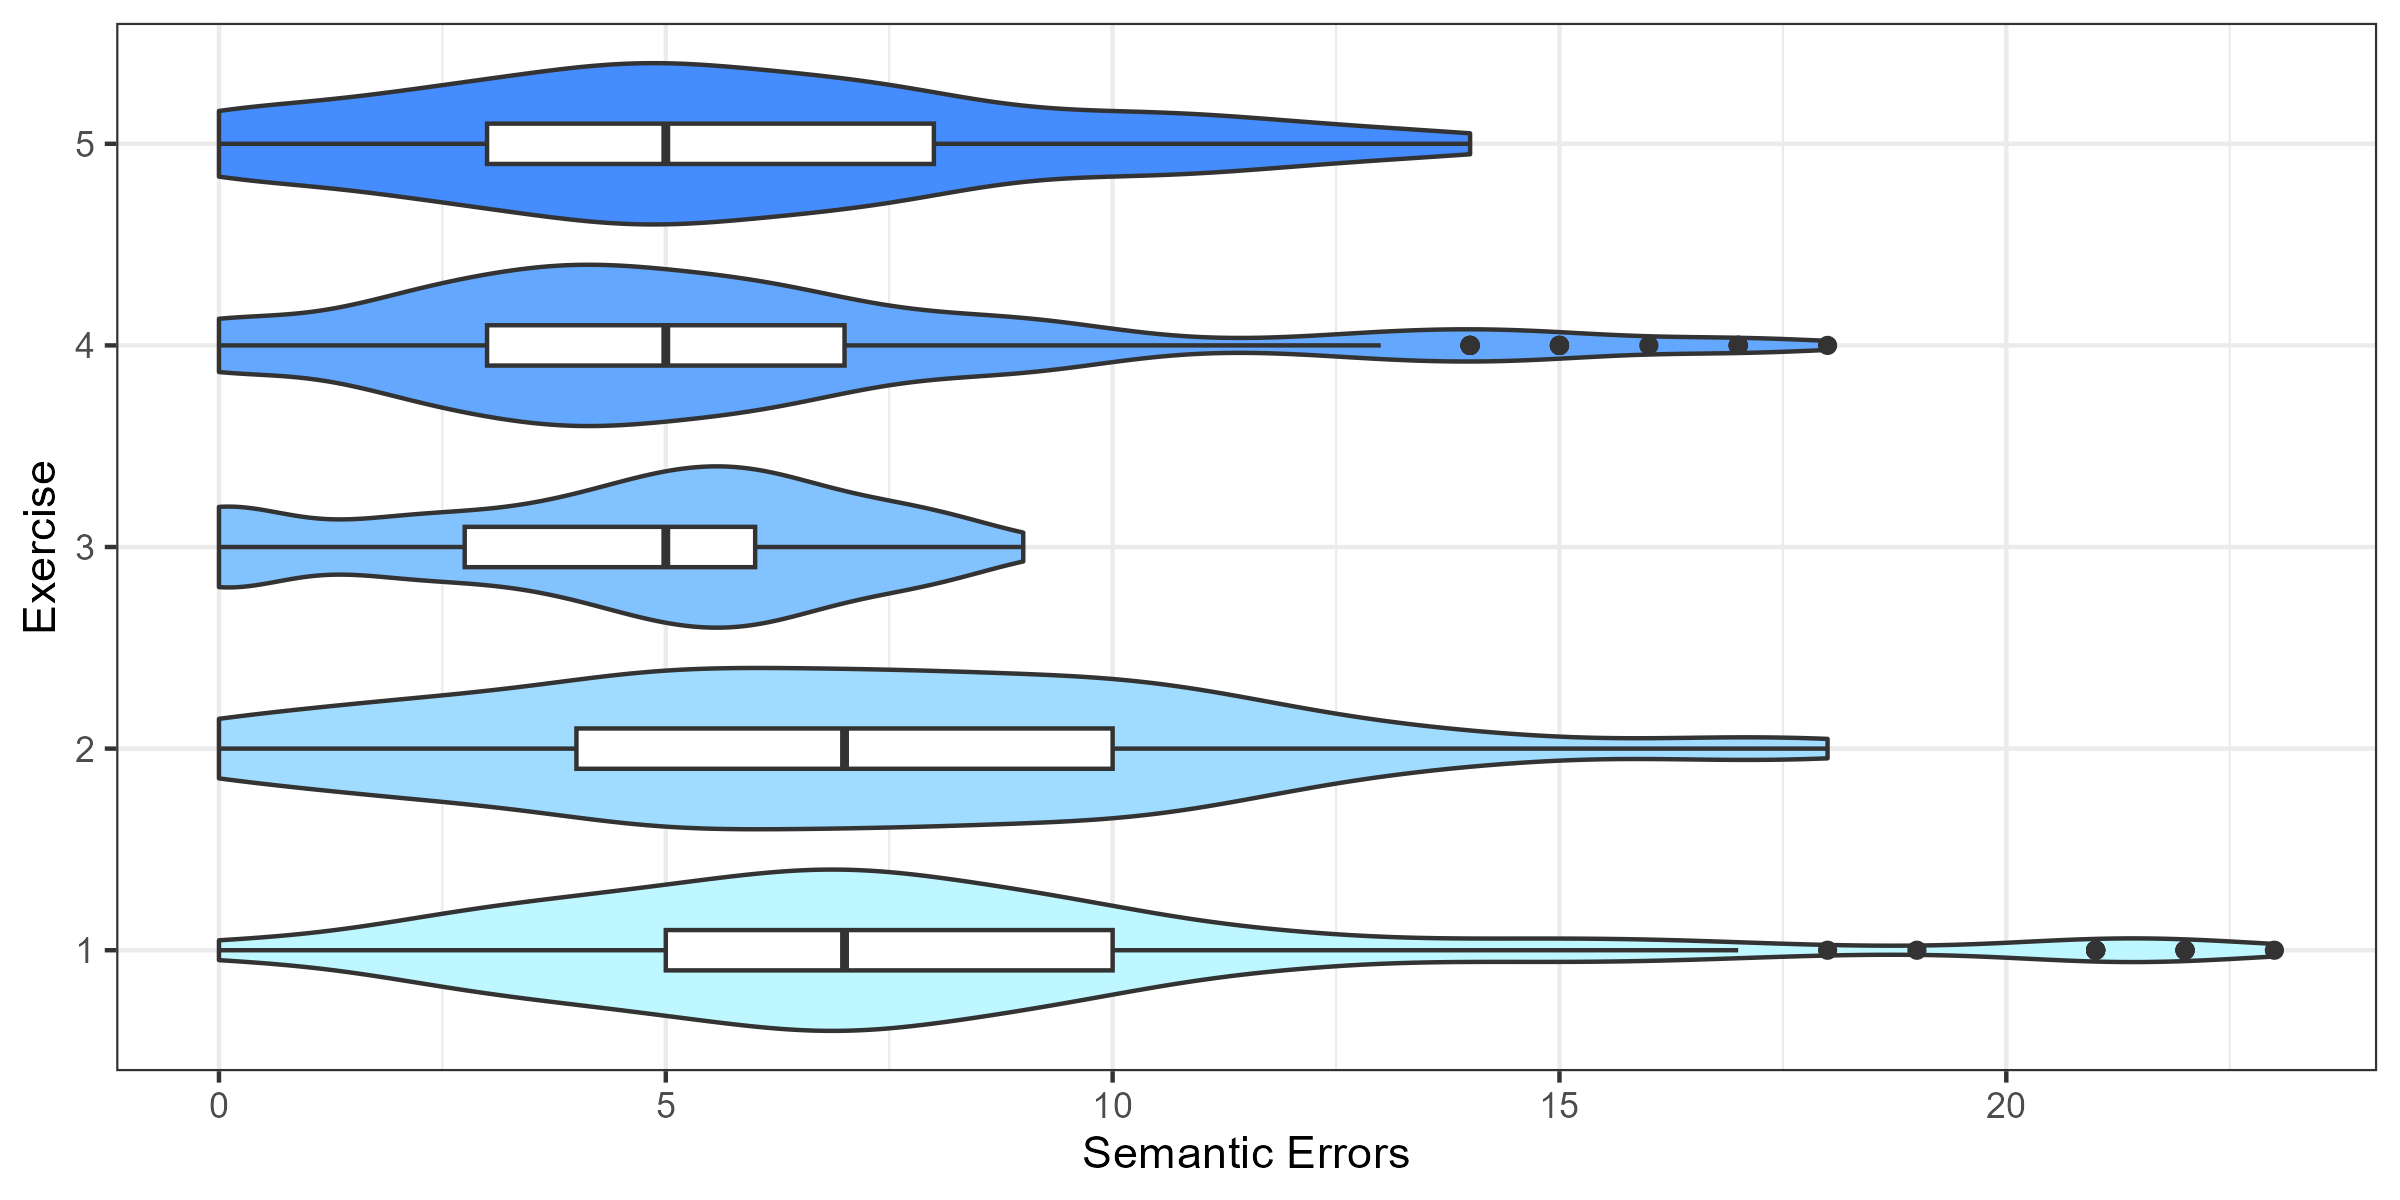
\includegraphics[width=\linewidth]{Template_Latex_ScuDo_Tesi/Chapter5/sem_violin.png}
        \caption{Box and violin plot for the distribution of semantic error counts per exercise}
        \label{fig:rq2_5_sem}
    \end{subfigure}
    \caption{Box and violin plots for RQ2 metrics}
    \label{fig:rq2_5}
\end{figure}

The distribution of diagram completeness is overall quite positive, seeing that all exercises have at least 70\% completeness on average, and all of them excluding exercise 2 have at least 75\%, the acceptable threshold for an exercise to be considered completed, making it reasonable to assume that the average student has been able to complete four out of the five exercises. Syntax errors are on average quite low, particularly decreasing around halfway through the course before increasing with exercise 4, and semantic errors show a similar trend, falling when going from exercise 1 to 2 and then 3 to increase once more for the final, more complex, two exercises. 

The results of the statistical analysis performed to answer RQ2, a linear model using the first exercise as the reference, are presented in Table \ref{tab:rq2_5_start}; coefficients are interpreted as the difference in performance with relation to the start of BPMN-related activities in the course, where students have yet to practice: performance improvements are represented by positive coefficients for diagram completeness, signifying diagrams with more correct elements over time, and by negative coefficients for error counts, implying a better understanding of modeling conventions and a higher ability to represent domain-specific details.

\begin{table}[ht]
    \footnotesize
    \centering
    \caption{Coefficients and p-values for linear model using fixed reference encoding for each progress metric. Statistically significant p-values are in bold.}
    \begin{tabular}{lrrr}
    \toprule
    Exercise & Completeness & Syntax Errors & Semantic Errors  \\
    \midrule
    2 & -4.37 (\textbf{4.86e-3}) & -0.37 (1.01e-1) & -0.93 (\textbf{4.83e-3}) \\
    3 & 1.08 (4.87e-1) & -0.51 (2.38e-2) & -3.6 (\textbf{\textless{} 2e-16}) \\
    4 & 1.14 (4.63e-1) & 0.36 (1.15e-1) & -2.26 (\textbf{1.03e-11}) \\
    5 & 2.41 (1.20e-1) & 0.16 (4.92e-1) & -2.40 (\textbf{6.19e-13}) \\
    \bottomrule
    \end{tabular}
    \label{tab:rq2_5_start}
\end{table}

For what concerns diagram completeness, the only comparison with the first exercises to yield a statistically significant p-value is the one with the second exercise, with a negative coefficient signifying a drop in performance; while the comparisons with subsequent exercises have a positive coefficient, implying performance improvements over time when solving more complex exercises, the absence of statistical significance hinders the analysis' relevance.

Syntax errors show a similar result: the comparison with the third exercise yields a slightly significant p-value, which is however still higher than the adjusted coefficient  $\alpha_C$: while the negative coefficient implies that students manage to attain a good understanding of BPMN theory and modeling rules after enough use of a gamified tool, the absence of significance means that the result cannot be taken for granted.

Lastly, semantic errors paint a different picture, with all comparisons yielding a significant p-value and negative coefficients: the interpretation is that the use of gamification was effective in helping students learn how to handle domain constraints, by reducing errors such as incorrect ordering, assigning elements to the wrong actors, or mishandling message exchanges.

The second step of the statistical analysis performed to answer RQ2 was to perform a second linear model, this time with a progressive encoding where a given exercise is taken as reference and compared against the following one, leading to four comparisons that show relative improvements as additional topics are added and the exercise difficulty increases; Table \ref{tab:rq2_5_prog} summarizes the coefficients and p-values for the three RQ2 metrics.

\begin{table}[ht]
    \footnotesize
    \centering
    \caption{Coefficients and p-values for linear model using progressive encoding for each progress metric. Statistically significant p-values are in bold.}
    \begin{tabular}{lrrr}
    \toprule
    Exercise Pair & Completeness & Syntax Errors & Semantic Errors  \\
    \midrule
    Ex. 1 -> Ex. 2 & -4.37 (\textbf{4.86e-3}) & -0.37 (1.01e-1) & -0.93 (\textbf{4.83e-3}) \\
    Ex. 2 -> Ex. 3 & 5.55 (\textbf{4.58e-4}) & -0.14 (5.34e-1) & -2.69 (\textbf{8.33e-16}) \\
    Ex. 3 -> Ex. 4 & 0.06 (9.69e-1) & 0.87 (\textbf{1.33e-4}) & 1.36 (\textbf{3.85e-05}) \\
    Ex. 4 -> Ex. 5 & 1.27 (4.12e-1) & -0.20 (3.75e-1) & -0.14 (6.80e-1) \\
    \bottomrule
    \end{tabular}
    \label{tab:rq2_5_prog}
\end{table}

Regarding diagram completeness and its relative progression, there is a positive improvement when going from the second to the third exercise with a statistically significant p-value, showing a substantial improvement around the middle of the course; however, the negative coefficient between the first and second exercise may also imply that exercises 2 and 3 had, in practice, difficulty levels different than what originally assumed, and that it would have been better to swap their position in the course to have a more reasonable challenge progression. Given the fact that results regarding correctness are mixed and most comparisons do not show statistical significance, null hypothesis ${H_{2.1_{0}}}$ cannot be rejected, since the improvements regarding diagram correctness over time are limited and not consistent enough.

For what concerns syntax errors, there is a statistically significant increase in the passage from the third to the fourth exercise: this exercise is the first to introduce advanced modeling concepts such as message exchanges and events, together with multiple-pool interaction, as part of the intended solution rather than an alternative option, making understanding of the associated rules a mandatory skill needed to complete the exercise. Overall, the presence of just one small statistically significant improvement and one negative effect makes it not possible to reject ${H_{2.2_{0}}}$: the effects of long-term gamification use has mixed effects on syntax knowledge acquisition for students.

Finally, the pairwise comparison between exercises shows a statistically significant reduction in semantic error counts when moving from the second to the third exercise followed by a significant increase when reaching the fourth exercise; the increase in errors for the latter pair is consistent with advanced concepts becoming mandatory for successfully completing an exercise, and the reduction of errors, while not significant, can also be observed when reaching the final exercise, showing that students managed to learn how to handle advanced concepts. The results are overall positive, showing that gamification definitely leads to a reduction in semantic errors with relation to the beginning of the course, and also causes improvements over time; as a consequence, ${H_{2.3_{0}}}$ can be rejected.

\answer{RQ2}{Applying gamification over time yielded mixed results: diagram correctness improved over time, albeit not in a statistically significant manner, and the order of two exercises with a different practical difficulty level than originally expected also caused a significant drop in performance for the second exercise. Similarly, the number of syntax errors was also not affected in a specifically positive or negative way, with a reduction halfway through the course and a subsequent increase once advanced topics became mandatory for completion. In turn, semantic comprehension benefited greatly from the longitudinal use of BIPMIN, with significant reductions in error counts for all exercises in comparison to the beginning of the course, and a moderate increase with the introduction of complex topics.}

A questionnaire was provided at the end of the course to collect the students' perception of the longitudinal experience, and answer the sub-questions that compose RQ3. RQ3.1 dealt with the students' perception of the BIPMIN tool's usability and was measured with the TAM questionnaire, used to assess the general perception of the tool, as well as with the GAMEX questions to measure how students interacted with the tool during the course. The latter questionnaire was included as a particularly important set of questions, given its inclusion in the original 2023 empirical study: given the neutral results obtained with the original study, the intention was to observe whether the improved version would be able to achieve a better distribution of the students' opinions, justifying the tool's rework. The distribution of answers to both questionnaires, computed as the average answer given by students for each construct of the questionnaires, can be seen in Figure \ref{fig:rq3_5}.

\begin{figure}[H]
    \centering
    \begin{subfigure}{0.5\linewidth}
        \centering
        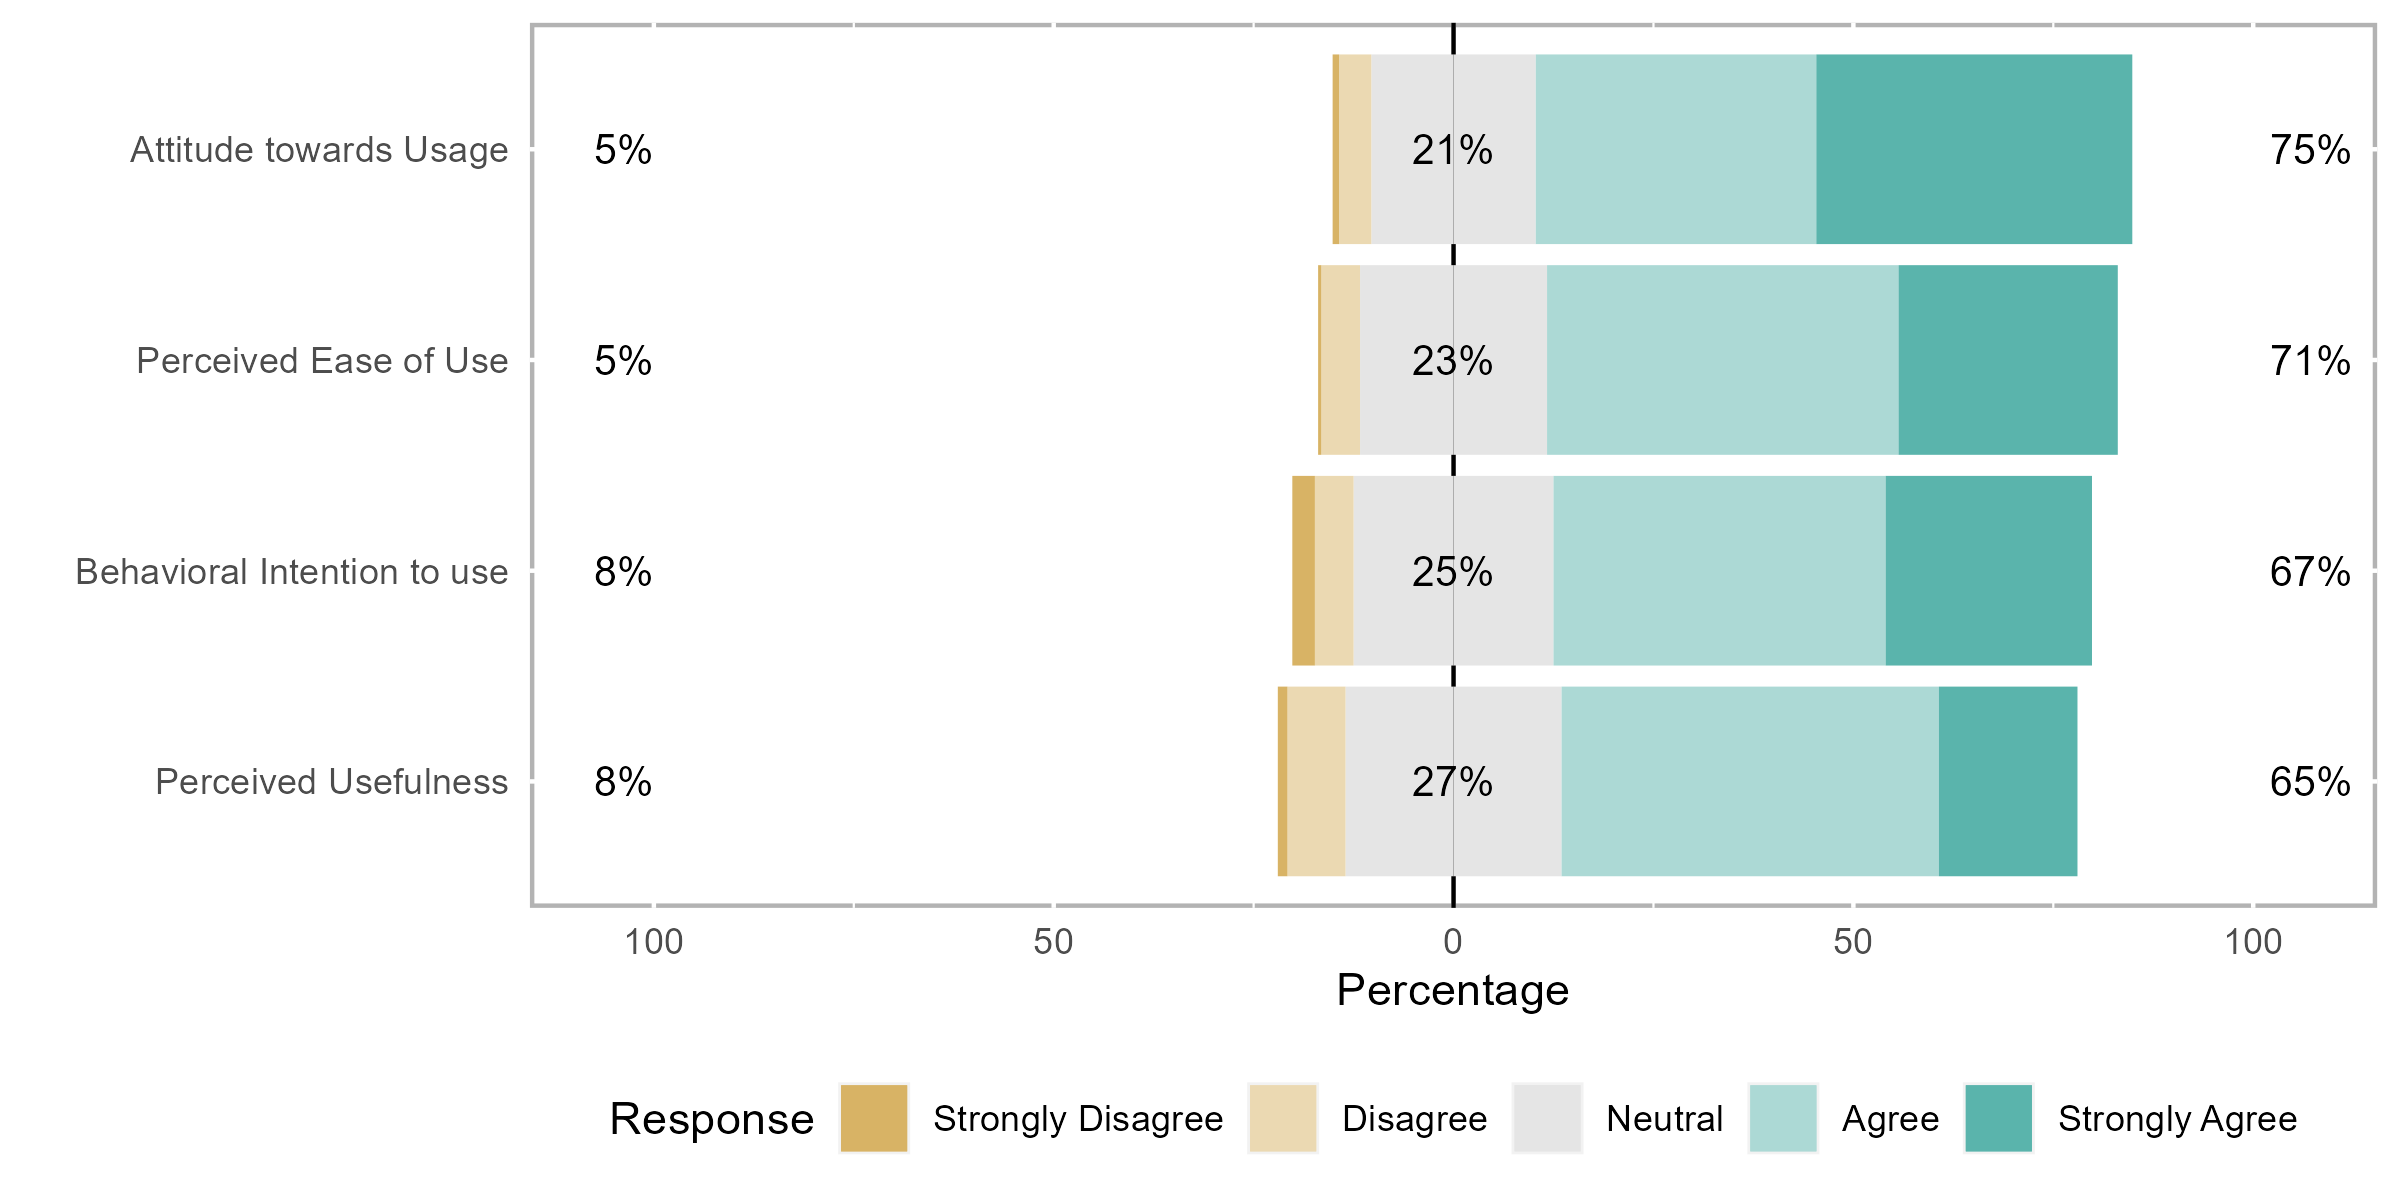
\includegraphics[width=\linewidth]{Template_Latex_ScuDo_Tesi/Chapter5/tam_plot.png}
        \caption{Distribution of answers to the TAM questionnaire}
        \label{fig:rq3_5_tam}
    \end{subfigure}\hfill
    \begin{subfigure}{0.5\linewidth}
        \centering
        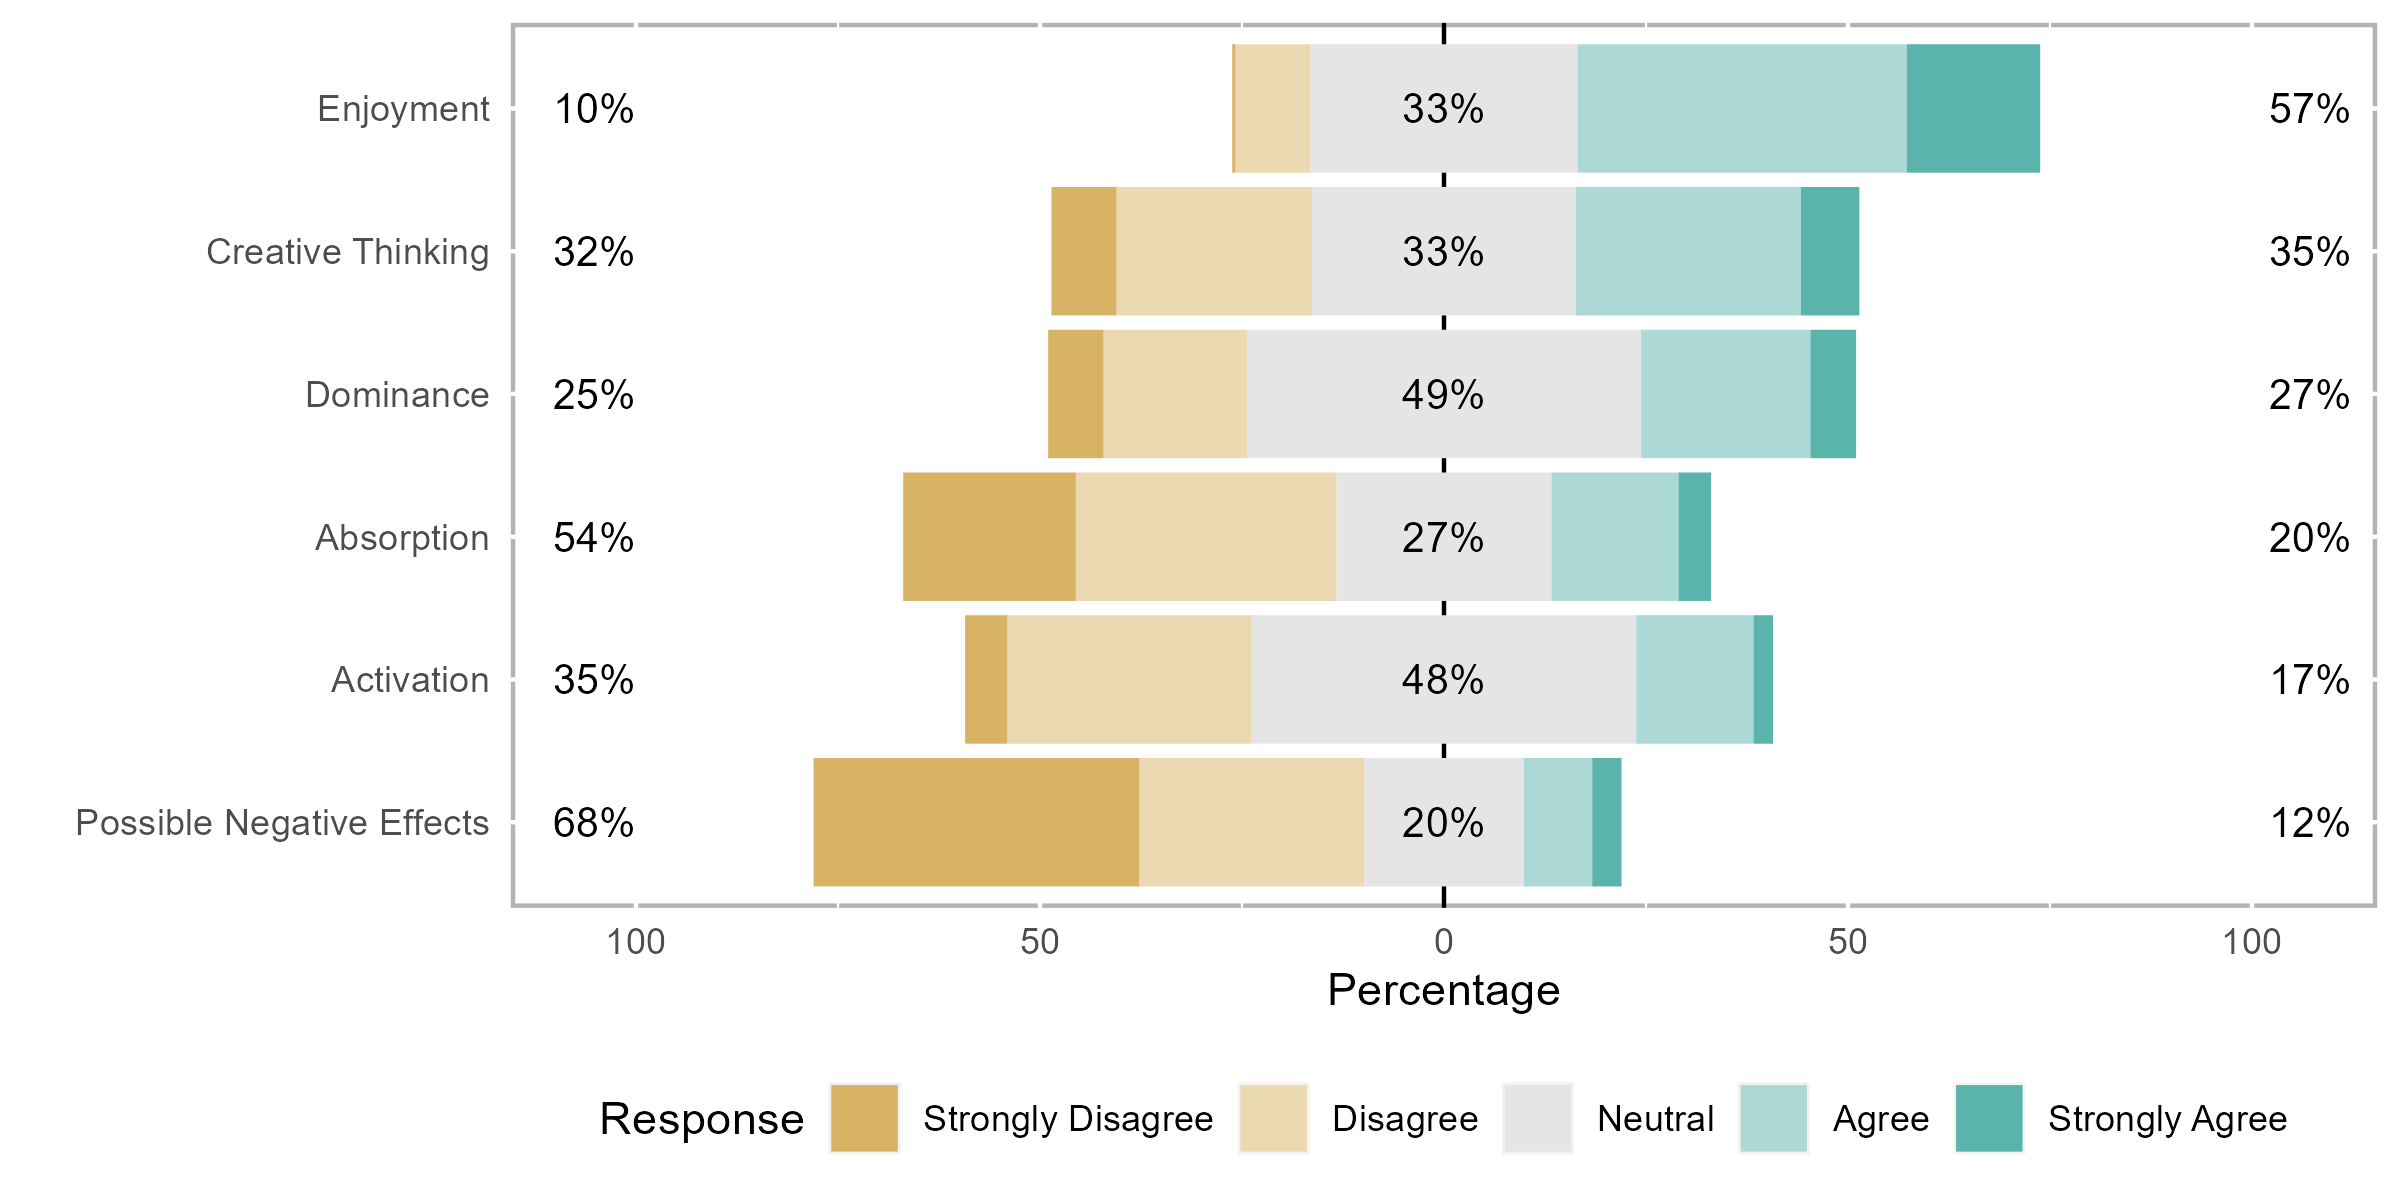
\includegraphics[width=\linewidth]{Template_Latex_ScuDo_Tesi/Chapter5/gamex_plot.png}
        \caption{Distribution of answers to the GAMEX questionnaire}
        \label{fig:rq3_5_gamex}
    \end{subfigure}
    \caption{Distribution of students' average opinions for RQ3.1 constructs}
    \label{fig:rq3_5}
\end{figure}

Answers given to the TAM questionnaire are overall, quite positive: all four constructs obtained a positive assessment according to at least 65\% of the students, highlighting a satisfactory implementation and presenting an easy to use application. The \textit{Attitude towards Usage} construct is particularly encouraging, with three quarters of the students expressing a favorable general opinion, implying that most students were encouraged to use BIPMIN and, consequently, to perform modeling assignments. The low negative scores for the two lesser ranked constructs (\textit{Behavioral Intention to Use} and \textit{Perceived Usefulness}) remain at a reasonable 8\%: the resulting interpretation is that most of the students believed that gamification was an effective and interesting addition to the BPMN modeling part of the course.

The distribution of answers given to the GAMEX questions is also a positive result: a noteworthy result is the fact that \textit{Enjoyment}, the third ranked construct in the original study, became the most appreciated one with 57\% of the students having a positive opinion, meaning that the revised BIPMIN made the modeling experience much more enjoyable compared to the prototype. Other constructs that were originally identified such as \textit{Creative Thinking} and \textit{Dominance} also saw an overall improvement, moving from 25\% and 22\% to 35\% and 27\% respectively: while these values are still not particularly high, the relative improvement means that at least one of the original limitations was overcame, since the tool now allowed for more freedom of action and student control than before. Lastly, \textit{Possible Negative Effects} remained the construct with the highest percentage of disagreeing students, a positive result given its negative connotation, meaning that the new version managed to keep the friendly and non frustrating user experience of the original version.

\answer{RQ3.1}{The answers to the TAM questionnaire show that BIPMIN was perceived as an easy to use tool by the students, with most of them agreeing on its usefulness in the context of modeling education. Most of the limitations that emerged from the answers given to the GAMEX questionnaire in the original 2023 study were resolved with the revised version, with enjoyment becoming a much more appreciated construct and the freedom of action and support for creative thinking also improving; the originally low perception of negative effects such as frustration and hostility was also confirmed with the new version, signifying an effective rework that addressed limitations found in the students' perception of the original prototype.}

RQ3.2 was measured with a set of questions focused on the game mechanics, similar to those used for the 2024 UMLegend study described in Chapter 4: for these questions, the average answer was computed for each game mechanic, while considering the opposite answer for the question related to the distracting effect, due to its negative connotation; the distribution of answers related to the mechanics is shown in Figure \ref{fig:rq32_5_mechs}.


\begin{figure}[ht]
    \centering
    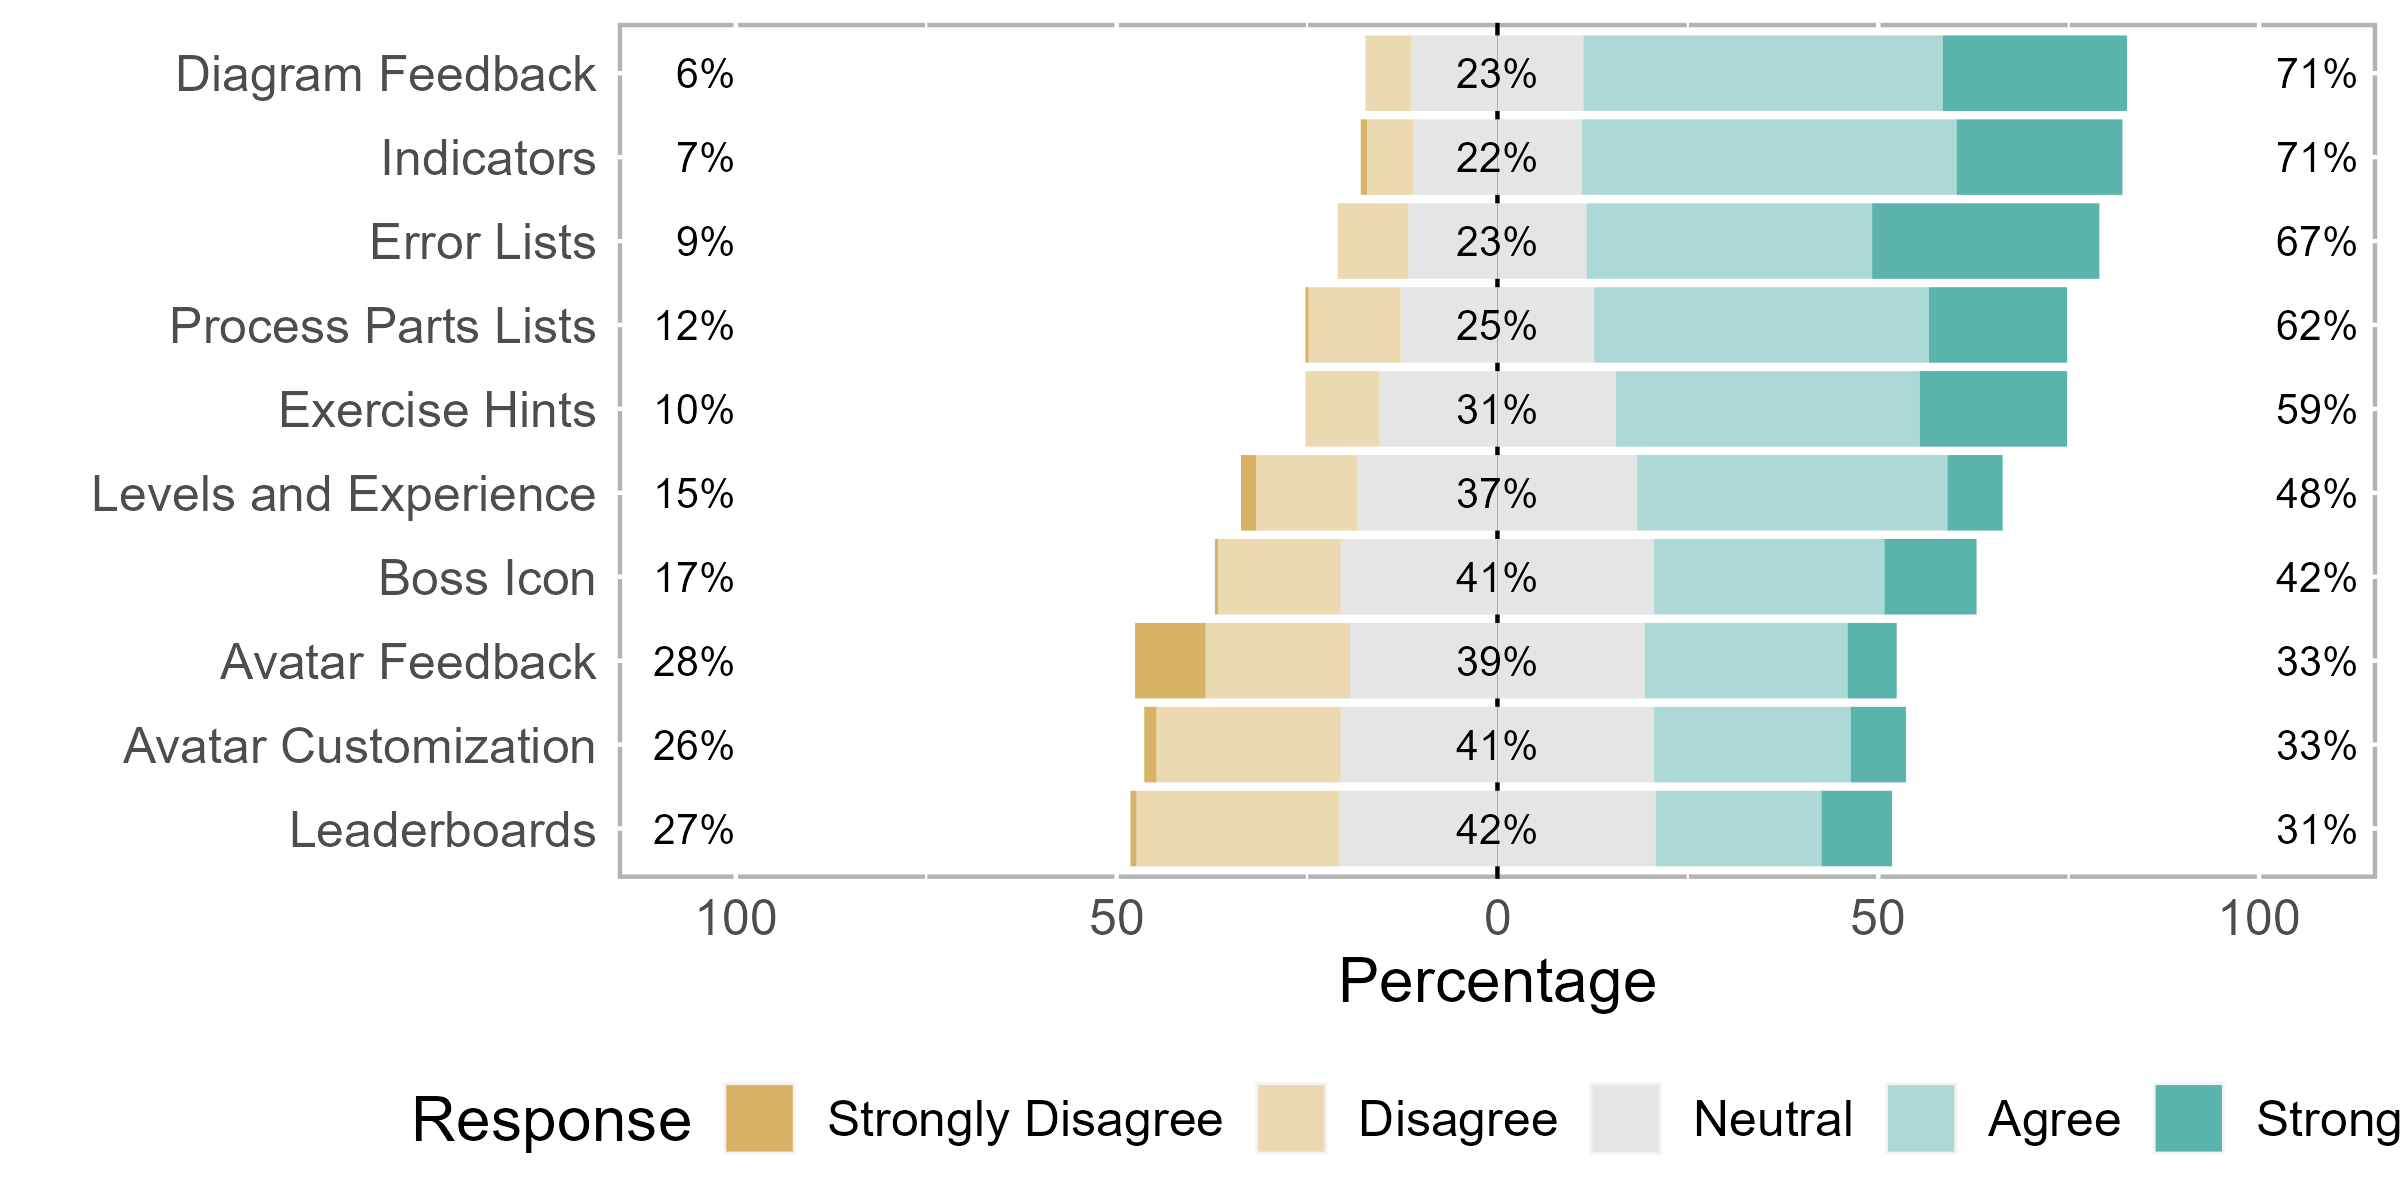
\includegraphics[width=1\linewidth]{Template_Latex_ScuDo_Tesi/Chapter5/mechs_plot.png}
    \caption{Distribution of answers related to the different game mechanics}
    \label{fig:rq32_5_mechs}
\end{figure}

The distribution of answers is overall quite positive, with half of them obtaining at least 50\% positive answers, and with the three mechanics with the lowest appreciation score still achieving success with around one third of the students. In line with the results obtained in the 2023 study with the questions related to game mechanics, the two most appreciated elements are diagram-based feedback and indicators, reinforcing the idea that direct, actionable assistance whose purpose is to guide students toward correct modeling is an effective and appreciated strategy to adopt in a gamified tool. The three mechanics that obtained a similarly positive score are also mechanics that reinforce this concept: error lists were appreciated by two thirds of the students, and feedback lists and hints are also worth noting due to having only 10\% of negative opinions, with the latter also obtaining a total of 0\% of \textit{Strongly Disagree} average score, showing the importance of supporting mechanics that replace human assistance in a longitudinal context, one of the original goals behind the development of the gamified tools described in these chapters. Lastly, the low appreciation of the longitudinal mechanics such as avatar customization and leaderboards is somewhat surprising since these mechanics were not present in the 2023 study and were better received in the single-session UMLegend study than in the longitudinal one: a possible interpretation may come from the division into a relative leaderboard and one showing the top students in the BIPMIN tool, while UMLegend showed all students together. Not having any indication of one's standing among the entire classroom may have made the mechanic feel less motivating; furthermore, the risk of leaderboards losing novelty over time may also be a reason to consider for the relatively low appreciation.

Regarding the students' perception of the longitudinal effects of BIPMIN, a total of four questions were included in the questionnaire: no average value was computed for these questions, taking each student's answers to compute the distribution of opinions, which is shown in Figure \ref{fig:rq32_5_long}.


\begin{figure}
    \centering
    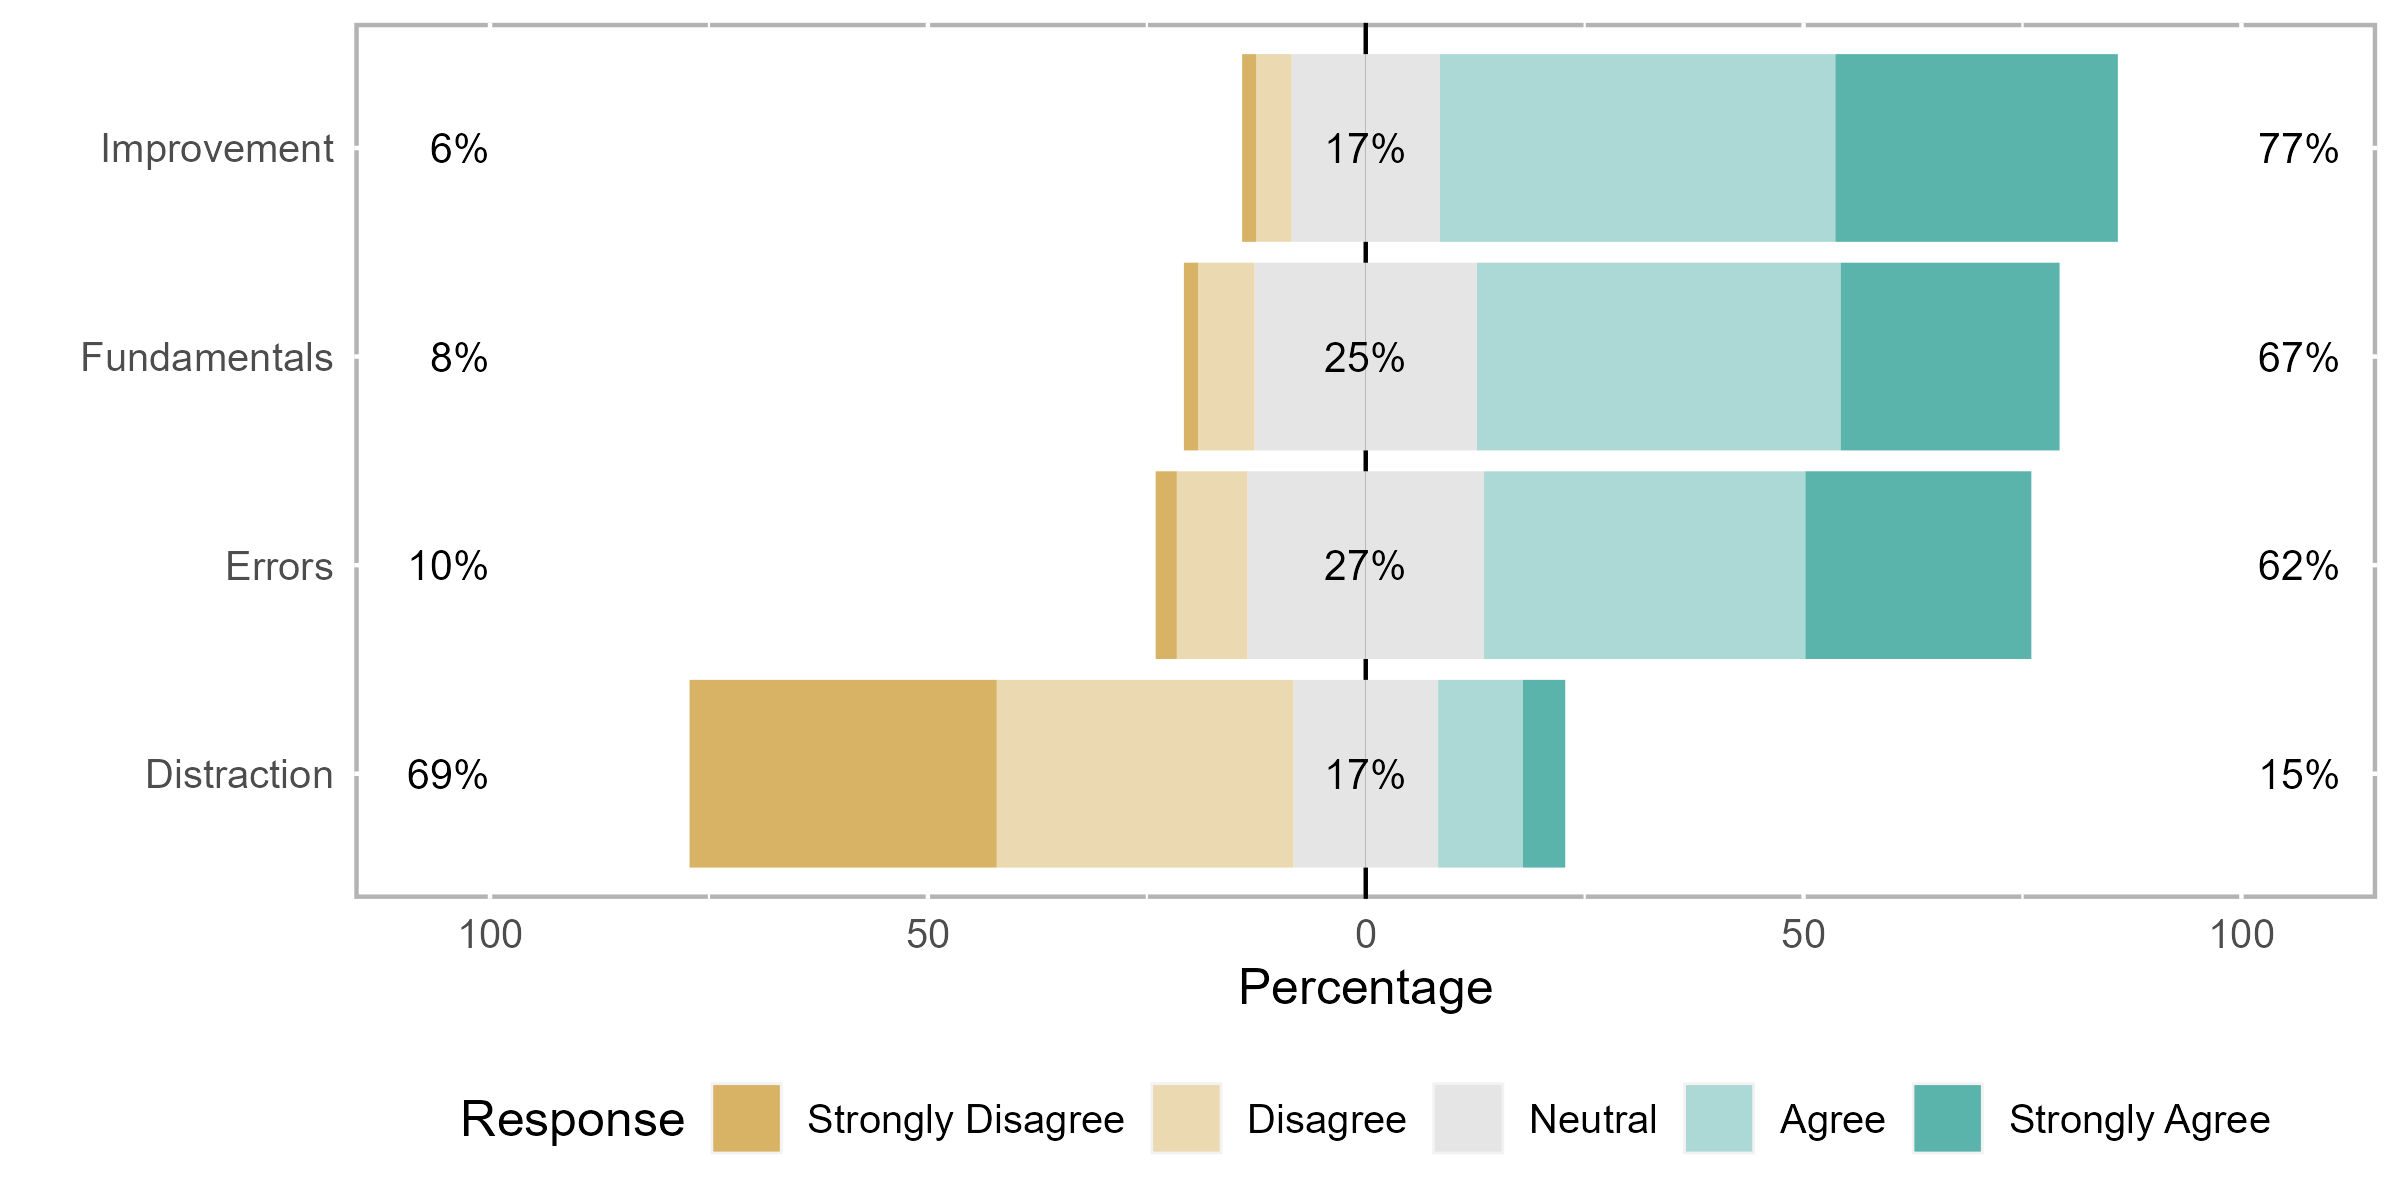
\includegraphics[width=1\linewidth]{Template_Latex_ScuDo_Tesi/Chapter5/long_plot.png}
    \caption{Distribution of answers related to the longitudinal usage of BIPMIN}
    \label{fig:rq32_5_long}
\end{figure}

All four answers show a general positive trend among students: most of them felt that, by using BIPMIN, they managed to learn the fundamental modeling rules and concepts, and 77\% of them stated their belief that continuous use of the tool helped them improve their knowledge. A vast majority of the students also stated that BIPMIN was not their sole focus during the course, and that the gamified tool did not distract them from other activities.

\answer{RQ3.2}{The students' perception of the game mechanics was mostly positive, and confirmed the findings of the original 2023 study: the most effective mechanics are those that guide them toward completion and help them understand good modeling practices by pointing out errors and correct choices; the relatively low appreciation of mechanics conceived for long-term use in a longitudinal context implies a need to redesign them for future use. The perception of longitudinal use was also positive, since students felt the positive effect of the tool for learning modeling practices, the reasons behind errors, and low distracting effect making sure BIPMIN was not the sole focus of the learning process, allowing for interaction with other topics as well.}

Lastly, two open questions were included to answer RQ3.3, with one of them asking for suggestions about possible improvements and another asking for how to better integrate BIPMIN in the course activities; following the open coding process, a total of 138 answers to the first question and 99 for the second were found to contain no suggestion, and were thus not considered. The set of topics found in the two questions can be seen in Figures \ref{fig:rq3_3_5_impr} and \ref{fig:rq3_3_5_integ}.


\begin{figure}[H]
    \centering
    \begin{subfigure}{0.5\linewidth}
        \centering
        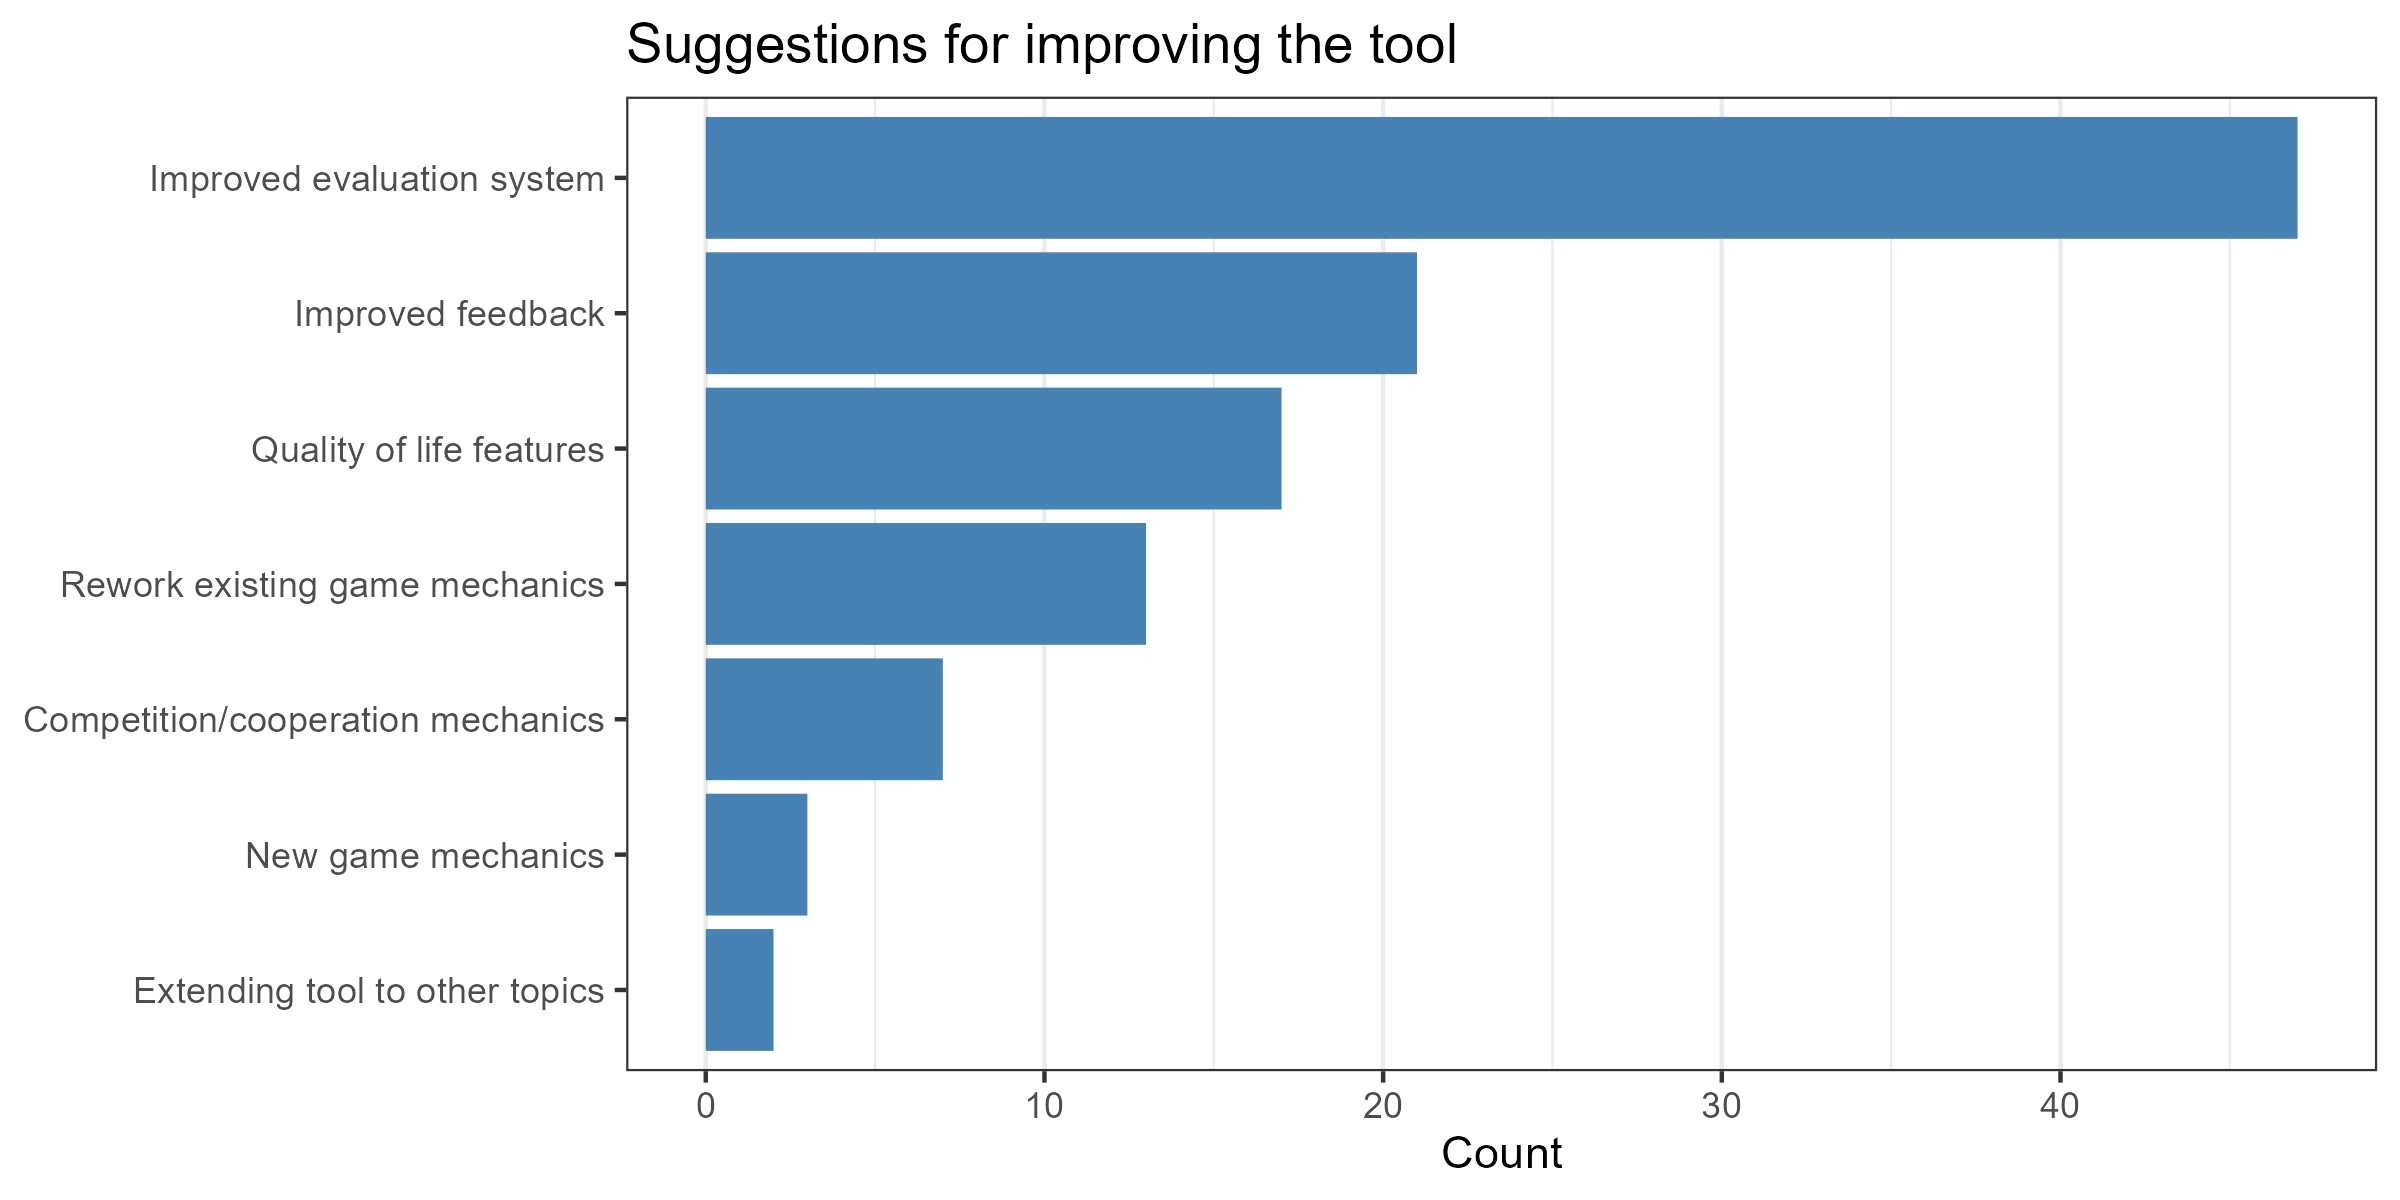
\includegraphics[width=\linewidth]{Template_Latex_ScuDo_Tesi/Chapter5/impr_plot.png}
        \caption{Student suggestions related to improvement areas}
        \label{fig:rq3_3_5_impr}
    \end{subfigure}\hfill
    \begin{subfigure}{0.5\linewidth}
        \centering
        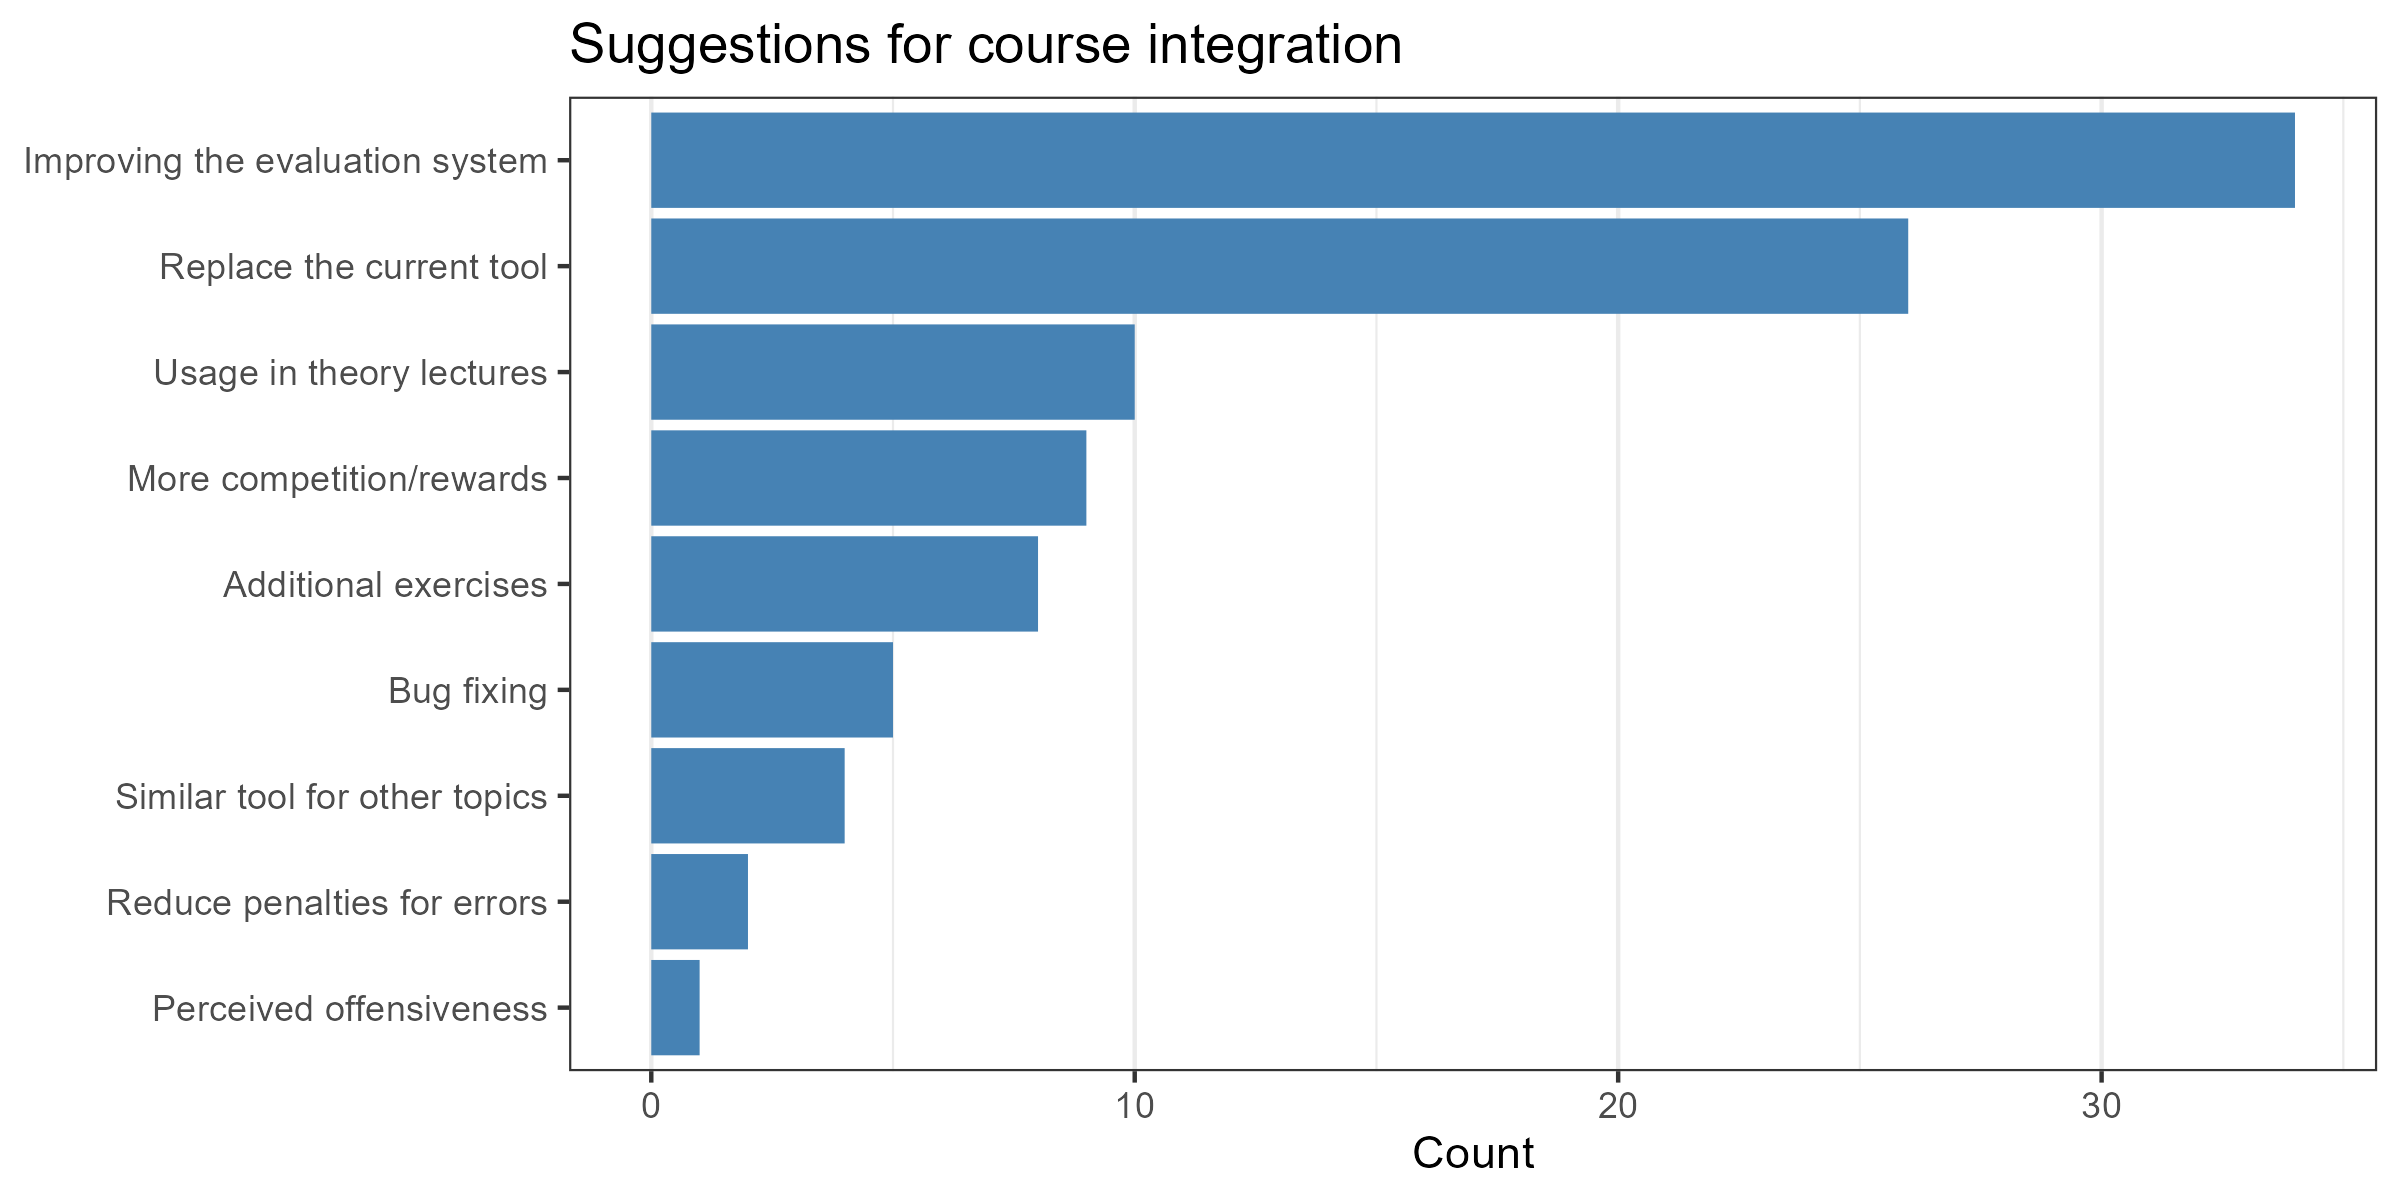
\includegraphics[width=\linewidth]{Template_Latex_ScuDo_Tesi/Chapter5/integ_plot.png}
        \caption{Student suggestions related to course integration}
        \label{fig:rq3_3_5_integ}
    \end{subfigure}
    \caption{Results of the open coding procedure on the answers given to the two open-ended questions}
    \label{fig:rq3_3_5}
\end{figure}

For what concerns improvement areas, the most common suggestion is to improve the evaluation engine, with 47 students asking for such a change: while the new version used for the longitudinal study was completely reworked to be more flexible and better identify errors and correct modeling choices, certain limitations were still in place, particularly for what concerns the need of synonyms to express element names. Live observation of the tool during lab activities showed multiple cases where students would use semantically correct phrases to label names and still receive no match due to certain words not being recognized (e.g., a task labeled \textit{Apply for internship} in the reference solution with \textit{Ask for internship} as a valid synonym represented with \textit{Request internship} not marked as a match due to the label not being included in the structure); this can be seen less as a limitation of the evaluation engine and more of a limitation in the solution definition approach, which requires teachers to identify as many variants as possible to express the same set of requirements. Other suggestions focused on enhancing the feedback even further, reworking game mechanics by adding competition and cooperation elements, or quality of life features such as automatic saving, allowing to see an exercise's requirements together with the modeler, or sharing diagrams with the teachers to receive direct comments.

Regarding suggestions for better course integration, the most common suggestion was once more related to the evaluation engine, highlighting the need of a more careful definition of the reference solutions to improve the students' learning experience; other relevant suggestions depended on the dissonance between practical exercises and the rest of BPMN-related activities such as theory lectures and the project work, which were performed with the non-gamified Signavio Academic platform. Many students reported the wish of a more complete integration of the gamified approach, including some asking for similar tools for the other modeling assignments, suggesting the need to integrate the two developed tools into a single platform.

Finally, one student raised a critical issue by stating the avatars' implementation as stereotyped and, in their interpretation, offensive: the randomly generated starting avatar was criticized with \textit{the effort to create more representation was just a very generalized approach which made me feel very stereotyped as an Arab woman who doesn't come from a Muslim nor African background}. Future work on the tool will require attention to how avatars are managed, perhaps with the introduction of a default state for avatars or with stylized, non-human options, to ensure the experience is as inclusive as possible and does not reinforce biases or stereotypes.

\answer{RQ3.3}{The students' suggestions highlighted that the evaluation engine, while improved from the original implementation, still needs attention and development efforts, mainly from the point of view of how solutions are defined, in order to ensure most of the alternative options are covered. Adopting a gamified tool for practical assignments only, while performing theory lectures and group activities with a different tool also led to a dissonant situation, making students wish for gamification to be applied to the entire course curriculum, including lectures and other modeling notations. Lastly, the avatar system may risk to reinforce stereotypes and appear as offensive to students, implying careful corrective actions to make the user experience more inclusive.}


\subsection{Threats to Validity}

The threats to validity for the longitudinal study are discussed in this section following the taxonomy introduced in Section \ref{sec:empirical_methods} \cite{wohlin2012experimentation}.

\textbf{Threats to internal validity:} the students' background and abilities may have influenced the grades and the metrics achieved in the exercises; the constant increase in the five exercises' difficulty has been applied to mitigate the threat, trying to ensure that students could manage solving harder exercises by acquiring skills during the course. The comparison of grades between different academic years also introduces a threat due to differences over the student cohorts: regarding the exam grades, the format of the questions was kept as similar as possible between the years to ensure consistency; the project work, instead, was executed differently in the 2023 course, where it was an individual assignment, while the 2024 project work was performed in student groups. Grades were normalized to account for the different formats, but this may still have influenced the distribution of project scores. Additionally, students may have had previous knowledge of BPMN modeling, potentially impacting their grades and their scores in the exercises; this latter threat is something that could not have been tested and accounted for.

\textbf{Threats to external validity:} the results have been obtained in the context of a Masters' course, it may not be possible to generalize the findings to other learning environments or to professional/industrial environments.

\textbf{Threats to construct validity:} learning outcomes were assessed with grades of two specific learning activities, other measures such as periodic assessments throughout the course may have also been valid to represent knowledge progression. For what concerns progression over time with diagram-related metrics, other criteria to measure diagram correctness may have also been used, as well as different semantic rules in addition to the ones implemented in the automatic evaluator.

\textbf{Threats to conclusion validity:} the Wilcoxon tests performed to answer RQ1 are non-parametric, and thus have no statistical prerequisite. The linear mixed models used to answer RQ2 are parametric: while these models are robust enough to tolerate moderate departures from normality, given the sample sizes involved in the analysis, the assumption cannot be formally verified and constitutes a residual threat. The analysis performed for RQ2 also assumed that all exercises were performed in their intended order, but there may have been students who tried them differently.

\subsection{Key findings and lessons learned}

The longitudinal study with the new version of BIPMIN was conducted to conclude the work described in the two preceding chapters, by describing the revised version of the tool developed in parallel with another tool according to the same design choices, trying to address and overcome the limitations emerged with the 2023 study. The experiment was conceptualized with the goal of verifying whether gamified BPMN modeling education, which had shown promising results in a single session compared to classical modeling, could maintain similarly good result and lead to improvements in the students' performance and their perception of the topic.

Continuous exposure to a gamified tool led to positive student reception, with the tool being perceived as more useful, enjoyable, and effective compared to its earlier version, whose student appreciation was more toward the neutral side. While students appreciated more the tool, game mechanics intended for long term use did not achieve as much success as anticipated, hinting at the need of a redesign of such mechanics, perhaps with the introduction of social aspects that let students create their own sub-groups with private leaderboards, allowing for more direct competition, and collaboration mechanics may also be explored as a future option.

The assessment of the students' opinions also confirmed the perception of game mechanics that had emerged with the two studies described in Chapters 3 and 4: students preferred mechanics such as direct diagram feedback and feedback lists that could give precise guidance on the correct parts of their diagrams and the existing errors with suggestions on how to fix them; the development focus on expanding these mechanics is thus confirmed as a valuable addition, hinting that development of future gamified tools for software engineering education should focus on quality and specificity of feedback explanations with automated assessment of the students' produced artifacts in addition to competitive or cosmetic mechanics whose rewarding effect may fall short over time. 

Furthermore, gamification also brought benefits beyond higher student engagement with modeling assignments, leading to an increase in grades for BPMN tasks in the end-of-course evaluations, showing a valuable positive effect that suggests further study concerning gamification of modeling education. Educational benefits were also observed over time, with students improving their ability to represent correct diagrams compared to the beginning of the course and reducing the number of their errors, suggesting that, by using the tool, students were able to gain a correct understanding of BPMN fundamentals and to put those lessons learned to good use.

Not all limitations that had emerged with the 2023 study were completely addressed, however: despite a complete redesign, the evaluation engine remained a severe limitation, due to cases where semantically valid modeling choices were not accepted as matched because of lexical differences, varying phrases, or unexpected synonyms, causing a reduction in student engagement due to unfair penalization. A similar issue had been identified with the empirical study performed with UMLegend, signifying the necessity to enhance the two tools with new strategies to define solutions beyond the scope of what a limited group of teachers may expect as correct, as well as more detailed evaluation methodologies that exploit textual semantic matching to analyze student artifacts. The use of Large Language Models, with their ability to process, handle, and produce textual content may be an effective strategy to adopt, and research activities started towards the end of the longitudinal study to explore such capabilities and how to integrate them in the existing tools.

Lastly, the use of a gamified tool for a single course topic (and for practical assignments only) was identified by multiple students as a key area for improvement, mentioning the cognitive overhead caused by using different tools and having to adapt to them. The parallel development of the two tools was organized with the end goal of producing a single gamified environment able to support multiple software modeling notations concurrently: findings confirm the importance of this goal, and future research directions should be focused mainly on achieving the integration of these tools, together with the development of new ones for other relevant SE topics.  

\articleSummary{
color1
}{
Summary of the BIPMIN longitudinal study
}{
The longitudinal study performed with BIPMIN showed that gamification can help students improve their BPMN knowledge, leading to higher grades in advanced modeling tasks and better understanding of fundamental rules, as well as small improvements in performance over time, with fewer errors and higher diagram correctness. The long-term use of the tool was also better received by students compared to the original single-session study, with noticeable improvements on the perception of enjoyment and creative freedom; mechanics that have a direct impact on learning were confirmed as the most appreciated and effective, confirming the importance of clear feedback as the most effective aspects for gamified tools to focus on. However, the new evaluation engine still had certain limitations that hindered certain aspects of the students' experience, and warrant the exploration of other strategies to enhance the two tools, which should also converge into a single educational environment for complete classroom use.
}

\graphicspath{{Chapter5/}}